\chapter{Guidance and Controllable Generation}\label{ch:guidance}
Diffusion models are powerful generative frameworks. In the unconditional setting, the goal is to learn $p_{\text{data}}(\rvx)$ and generate samples without external input.

Many applications, however, require \emph{conditional generation}, where outputs satisfy user-specified criteria. This can be achieved by steering an unconditional model or directly learning the conditional distribution $p_0(\rvx | \rvc)$, with condition $\rvc$ (e.g., label, text description, or sketch) guiding the process.

This chapter builds on a principled view of the conditional score, which decomposes into an \emph{unconditional direction} and a \emph{guidance direction} that nudges samples toward the condition while preserving realism. We explain why guidance is essential, show how the conditional score serves as a unifying interface for control, and survey ways to approximate the guidance term. We then distinguish \emph{control} (meeting the condition) from \emph{alignment} (meeting human preference under the condition), and describe how preferences can be incorporated into the same framework. Finally, we discuss direct optimization of preference without additional reward models (i.e., a learned scorer that assigns higher values to outputs better aligned with human preference).








\clearpage
\newpage

\section{Prologue}\label{sec:prologue-guidance}


\begin{figure}[th!]
    \centering
    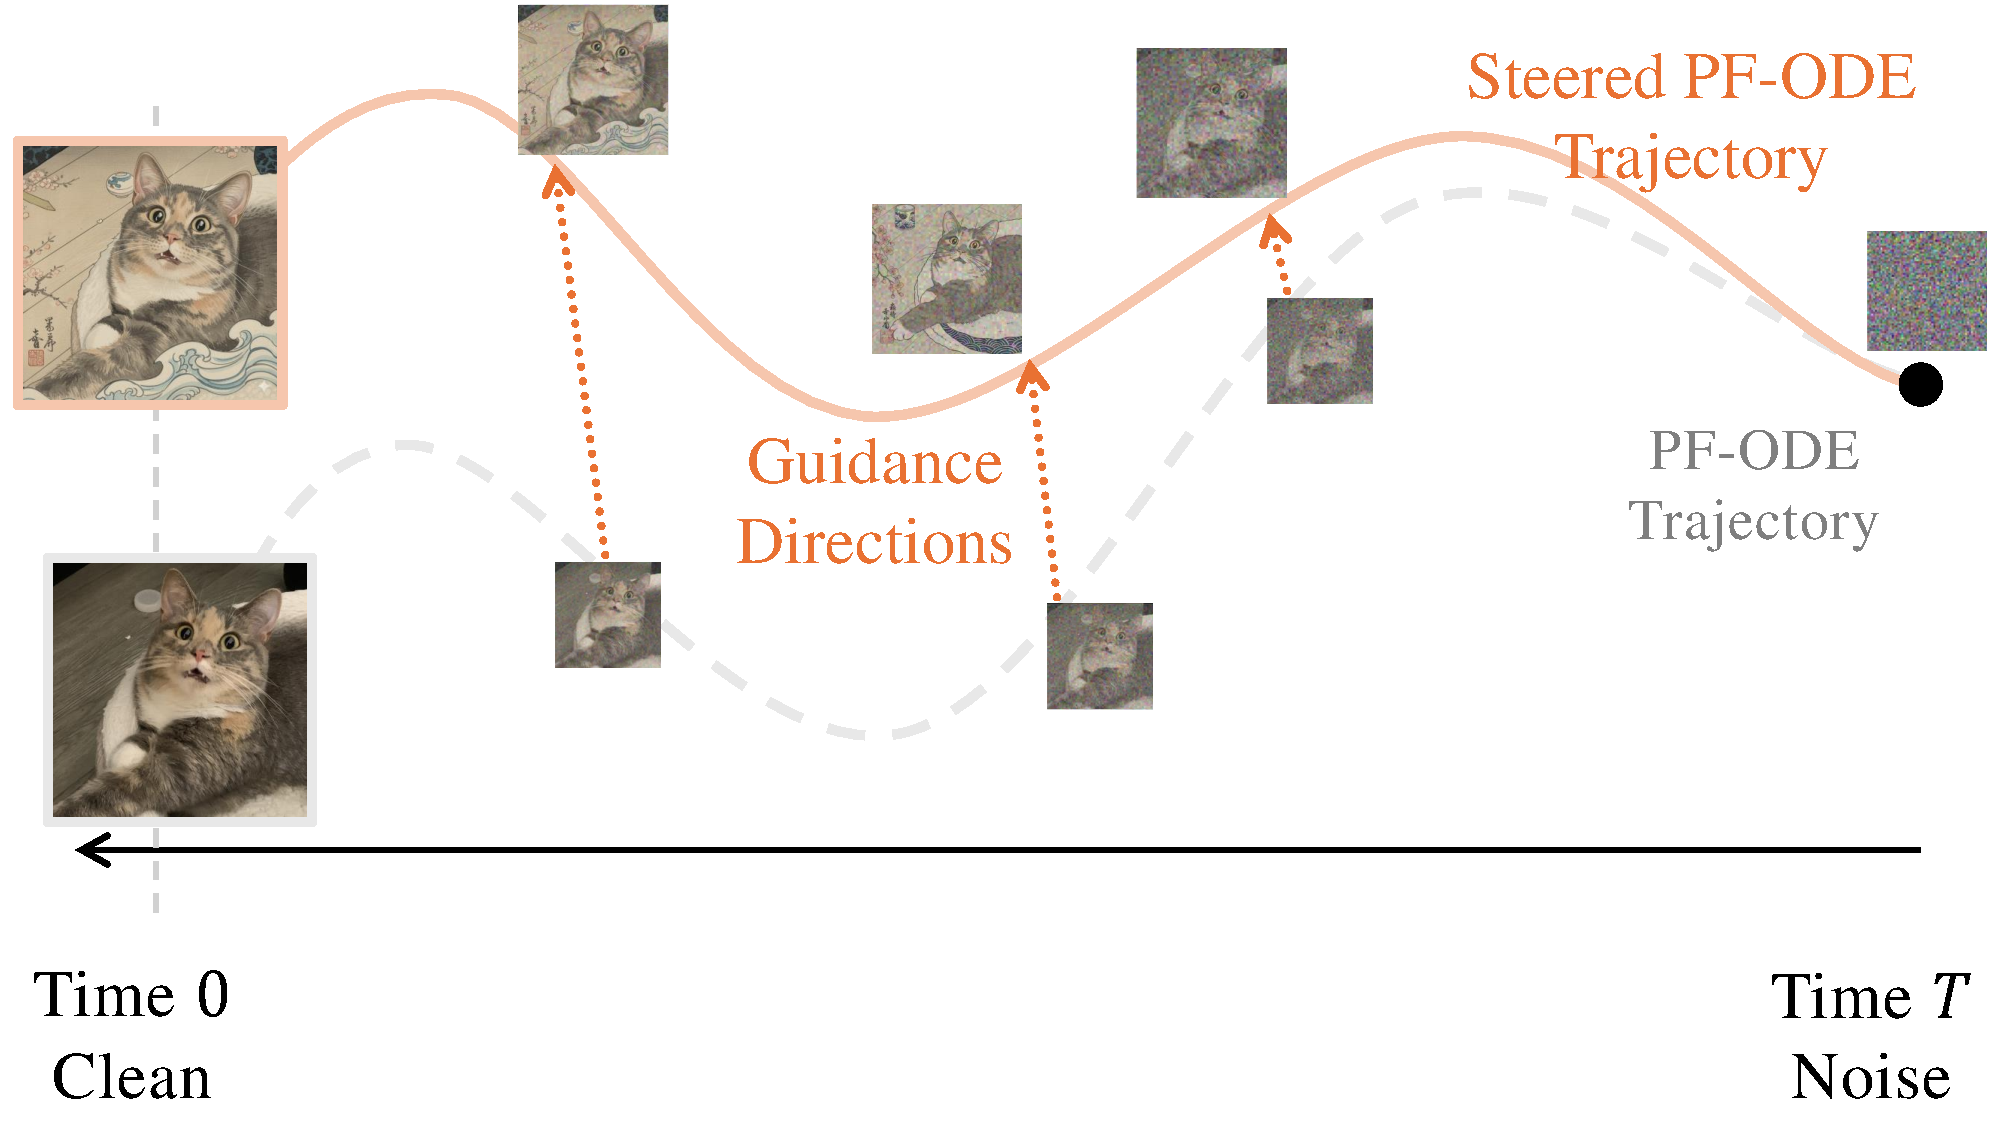
\includegraphics[width=\linewidth]{Images/PartC/guidance.pdf}
\caption{\textbfs{Illustration of steered diffusion sampling.}
Reverse-time PF-ODE sampling begins from pure noise at the right ($t = T$) and gradually evolves toward a clean sample at the left ($t = 0$). 
During this process, guidance directions $\nabla_{\rvx_t}\log \tilde{p}_t(\rvc |\rvx_t)$, weighted by $w_t$, modify the velocity field according to
$\nabla_{\rvx_t}\log p_t(\rvx_t) + w_t\,\nabla_{\rvx_t}\log \tilde{p}_t(\rvc |\rvx_t)$.
These additional directions steer the trajectory toward the desired attribute (Japanese painting style) while the sample is progressively refined from coarse to fine detail.
\figcredit{Created by the authors.}}
    \label{fig:guidance}
\end{figure}


The generation process of diffusion models proceeds in a coarse-to-fine manner, providing a flexible framework for controllable generation. At each step, a small amount of noise is removed and the sample becomes clearer, gradually revealing more structure and detail. This property enables control over the generation process: by adding a guidance term to the learned, time-dependent velocity field, we can steer the generative trajectory to reflect user intent.

A principled foundation for guidance-based sampling in diffusion models is the Bayesian decomposition of the conditional score. For each noise level $t$,
\begin{mdframed}
\begin{align}
\nabla_{\rvx_t}\log p_t(\rvx_t |\rvc)
=
\underbrace{\nabla_{\rvx_t}\log p_t(\rvx_t)}_{\text{unconditional direction}}
+
\underbrace{\nabla_{\rvx_t}\log p_t(\rvc |\rvx_t)}_{\text{guidance direction}}.
\label{eq:guidance_bayes}
\end{align}
\end{mdframed}
This identity shows that conditional sampling can be implemented by adding a guidance term $\nabla_{\rvx_t}\log p_t(\rvc |\rvx_t)$ on top of the unconditional score. A wide range of controllable generation methods (e.g., classifier guidance~\citep{dhariwal2021diffusion}, general training-free guidance~\citep{ye2024tfg}) can be interpreted as different approximations of this guidance term, since $p_t(\rvc |\rvx_t)$ is generally intractable due to marginalization over $\rvx_0$.

Once such an approximation is available, sampling simply replaces the unconditional score with its conditional counterpart. Using \Cref{eq:guidance_bayes}, the PF-ODE becomes
\begin{align}\label{eq:condition_prob_ode}
\begin{aligned}
    \frac{\diff \mathbf{x}(t)}{\diff t} &= f(t)\mathbf{x}(t) - \frac{1}{2} g^2(t) \underbrace{\nabla_{\rvx_t} \log p_t(\rvx(t) |\rvc)}_{\text{conditional score}} \\
    &= f(t)\mathbf{x}(t) - \frac{1}{2} g^2(t) \Big[ \nabla_{\rvx_t} \log p_t(\rvx(t)) + \nabla_{\rvx_t} \log p_t(\rvc |\rvx(t)) \Big].
\end{aligned}
\end{align}
We highlight that steering these time-dependent vector fields fundamentally relies on their linearity, so the discussion below, formulated in score prediction, naturally extends to $\rvx$-, $\beps$-, and $\rvv$-prediction through their linear relationships as in \Cref{eq:predictions-equivalence}.

\paragraph{Instantiations of the Guidance Direction.}
\begin{enumerate}[leftmargin=*]
\item \textbfs{Classifier Guidance (CG).} In \Cref{sec:cg}, classifier guidance (CG) trains a time-conditional classifier
$p_{\bpsi}(\rvc | \rvx_t, t)$ on noised data $\rvx_t$ (obtained by corrupting
clean labeled samples at level $t$). At sampling time, its input gradient
provides the guidance term:
\[
\nabla_{\rvx_t}\log p_{\bpsi}(\rvc | \rvx_t, t)
 \approx  \nabla_{\rvx_t}\log p_t(\rvc | \rvx_t),
\]
which is then added to the unconditional score~\citep{dhariwal2021diffusion}.
\item \textbfs{Classifier-Free Guidance (CFG).} In \Cref{sec:cfg}, CFG directly trains a single conditional model
\[
\rvs_{\bphi}(\rvx_t,t,\rvc) \approx \nabla_{\rvx_t}\log p_t(\rvx_t|\rvc),
\]
where the unconditional model is learned jointly by randomly replacing the condition with a special null token for a fraction of the training steps.
\item \textbfs{Training-Free (Surrogate) Guidance.}  The conditional $p_t(\rvc| \rvx_t)$ is generally intractable because it
requires marginalizing over the clean latent $\rvx_0$:
\[
p_t(\rvc| \rvx_t)
= \int p(\rvc| \rvx_0)  p(\rvx_0| \rvx_t)  \mathrm d\rvx_0,
\]
and, in typical applications, at least one of these factors is unknown, making the integral intractable.

In \Cref{subsec:tfg}, training-free (loss-based) guidance avoids evaluating the 
conditional likelihood $p_t(\mathbf{c}| \mathbf{x}_t)$ directly. 
Instead, it introduces an off-the-shelf loss $\ell(\mathbf{x}_t,\mathbf{c};t)$ 
and defines a surrogate conditional distribution $\widetilde p_t(\mathbf{c}|\mathbf{x}_t) $ as,
\[
\widetilde p_t(\mathbf{c}|\mathbf{x}_t) \propto \exp\!\big(-\tau\,\ell(\mathbf{x}_t,\mathbf{c};t)\big),
\quad \tau>0,
\]
which acts as a pseudo-likelihood. 
This formulation sidesteps the intractability of computing the true conditional 
likelihood while still enabling guidance through gradients of the chosen loss. Its conditional score is computed solely by the gradient of the loss with $\tau$:
\[
\nabla_{\rvx_t}\log \widetilde p_t(\rvc|\rvx_t)
= -\tau \nabla_{\rvx_t}\ell(\rvx_t,\rvc; t).
\] 
This term is added to the unconditional score with a guidance weight $w_t$:
\[
 \nabla_{\rvx_t}\log p_t(\rvx_t)
+ w_t \bigl[-\tau \nabla_{\rvx_t}\ell(\rvx_t,\rvc; t)\bigr].
\]
which is exactly the score of the \emph{tilted} density $\widetilde p_t^{\mathrm{tilt}}(\rvx_t| \rvc)$ defined as:
\[
\widetilde p_t^{\mathrm{tilt}}(\rvx_t| \rvc) \propto  p_t(\rvx_t) \widetilde p_t(\rvc| \rvx_t)^{w_t}
 \propto  p_t(\rvx_t) \exp\!\big(-w_t\tau \ell(\rvx_t,\rvc; t)\big).
\]
In practice, we replace the conditional score of sampling in \Cref{eq:condition_prob_ode} with this tilted score, and solving the resulting ODE to  draw samples.

In view of this, classifier guidance is simply surrogate guidance with a learned classifier $\widetilde p_t(\mathbf{c}|\mathbf{x}_t):=p_{\bpsi^\times}(\rvc| \rvx_t,t)$ via:
\[
\ell(\rvx_t,\rvc; t) = -\log p_{\bpsi^\times}(\rvc| \rvx_t,t), \quad \tau=1.
\]

The effect of guidance on the sampling trajectory is illustrated in \Cref{fig:guidance}.

All of these techniques can likewise be applied on top of a conditional model, 
allowing extra control signals to be injected during generation.

\end{enumerate}
\rmkb{Guided PF-ODE does \emph{not} sample from the tilted family (in general).
Even with exact scores and exact ODE integration, replacing the score by the
\emph{tilted} score does not make the time–$t$ marginals equal to
$\{\widetilde p_t^{\mathrm{tilt}}(\cdot|\rvc)\}_{t\in[0,1]}$, nor the terminal law equal to
$\widetilde p_0^{\mathrm{tilt}}(\cdot|\rvc)$. 

Define
\[
\rvv_t^{\mathrm{orig}} = \rvf - \tfrac12 g^2(t) \nabla \log p_t, \quad
\rvh_t(\rvx)=e^{-w_t\tau \ell(\rvx,\rvc;t)}, \quad
\widetilde p_t^{\mathrm{tilt}}=\tfrac{p_t \rvh_t}{Z_t}.
\]
The guided PF-ODE uses
\[
\rvv_t^{\mathrm{tilt}} = \rvf - \tfrac12 g^2(t) \nabla \log \widetilde p_t^{\mathrm{tilt}}
= \rvv_t^{\mathrm{orig}} - \tfrac12 g^2(t) \nabla \log \rvh_t.
\]

If $\widetilde p_t^{\mathrm{tilt}}$ were the true marginals, they would satisfy
\[
\partial_t \widetilde p_t^{\mathrm{tilt}} + \nabla\!\cdot(\widetilde p_t^{\mathrm{tilt}} \rvv_t^{\mathrm{tilt}})=0.
\]
But a direct calculation gives the residual
\begin{align*}
    &\partial_t \widetilde p_t^{\mathrm{tilt}} + \nabla \cdot(\widetilde p_t^{\mathrm{tilt}}  \rvv_t^{\mathrm{tilt}})
\\= &\widetilde p_t^{\mathrm{tilt}} \Big[ \partial_t \log \rvh_t
+ \rvv_t^{\mathrm{orig}} \cdot\nabla \log \rvh_t
- \tfrac12 g^2(t) \big(\Delta \log \rvh_t + \|\nabla \log \rvh_t\|^2 \big)
- \tfrac{Z_t'}{Z_t} \Big].
\end{align*}

Thus, $\widetilde p_t^{\mathrm{tilt}}$ coincides with the PF-ODE marginals if and only if the bracketed term vanishes for all $\rvx$, i.e.
\[
\partial_t \log \rvh_t + \rvv_t^{\mathrm{orig}} \cdot\nabla \log \rvh_t
= \tfrac12 g^2(t)\big(\Delta \log \rvh_t + \|\nabla \log \rvh_t\|^2\big) + \tfrac{Z_t'}{Z_t}.
\]
This condition holds trivially when $w_t\equiv 0$ (unconditional generation), but almost never for 
$\rvh_t(\rvx)=e^{-w_t\tau\ell(\rvx,\rvc;t)}$, except in very special cases of $w_t$ or $\ell$. Therefore, in general,
$\{\widetilde p_t^{\mathrm{tilt}}\}$ are \emph{not} the PF-ODE marginals, and terminal samples are \emph{not} distributed as $\widetilde p_0^{\mathrm{tilt}}(\rvx_0|\rvc)$. This perspective is also related in spirit to \citep{lai2023fp}.


For readers interested in going beyond this heuristic guidance, correction-based approaches~\citep{skreta2025feynman}, such as Feynman--Kac Correctors, aim to explicitly compensate for the mismatch between the guided dynamics and the desired tilted distributions, so that sampling follows the intended family more faithfully throughout the trajectory.

}




% If an additional attribute $\tilde{\rvc}$ is desired under a base condition $\rvc$, one can stacking or refining conditions
% \begin{align*}
%     \nabla_{\rvx_t}\log p_t(\rvx_t | \rvc,\tilde{\rvc})
% &=
% \nabla_{\rvx_t}\log p_t(\rvx_t | \rvc)
% +
% \nabla_{\rvx_t}\log p_t(\tilde{\rvc}| \rvx_t,\rvc)
% \\&\approx
% \rvs_{\bphi^\times}(\rvx_t,t,\rvc) - \nabla_{\rvx_t}\ell(\rvx_t,\rvc,\tilde{\rvc};t),
% \end{align*}
% so one can compose controls by adding further surrogate guidance terms.

\paragraph{From Control to Better Alignment with Direct Preference Optimization.}
Strong control can be on-condition but off-preference: a sample may satisfy the conditioning signal (e.g., the prompt) yet deviate from what humans actually prefer. We formalize this by \emph{tilting} the conditional target by a preference rating\footnote{We remark that the training-free guidance can also be viewed in the same framework of finding a tilted distribution with a guidance of loss $\ell(\rvx_t, \rvc, t)$}:
\[
\widetilde p_0^{\mathrm{tilt}}(\rvx_0| \rvc) \propto p_0(\rvx_0|\rvc) \exp \big(\beta r(\rvx_0,\rvc)\big),
\]
where $r(\rvx_0,\rvc)$ is a scalar alignment rating (reward) for a clean sample $\rvx_0$ and condition $\rvc$ (larger $r$ indicates better alignment).  In practice, $r$ may be (i) the logit or log-probability of an external reward/classifier, (ii) a similarity measure (e.g., CLIP/perceptual~\citep{radford2021learning}), or (iii) a learned preference model.

% \subparagraph{Training-Free Method and Its Relation to Training-Free Guidance.}
% At intermediate times, the tilted marginals $\tilde{p}_t(\rvx_t|\rvc)$ satisfy
% \[
% \nabla_{\rvx_t}\log \tilde{p}_t(\rvx_t|\rvc)
% =
% \nabla_{\rvx_t}\log p_t(\rvx_t|\rvc)
% +
% \nabla_{\rvx_t}\log \E \left[\exp \big(\beta r(\rvx_0,\rvc)\big) |dle|  \rvx_t,\rvc\right],
% \]
% where the conditional expectation is under the base posterior $p(\rvx_0|\rvx_t,\rvc)$. For small $\beta$, a first-order cumulant expansion gives
% \[
% \nabla_{\rvx_t}\log \tilde{p}_t(\rvx_t|\rvc)
% \approx 
% \nabla_{\rvx_t}\log p_t(\rvx_t|\rvc)
% + \underbrace{\beta \nabla_{\rvx_t}\E \left[r(\rvx_0,\rvc)|\rvx_t,\rvc\right]}_{\mathrm{alignment\ guidance}}
% \quad(+ \mathcal O(\beta^2)).
% \]
% Thus alignment guidance adds the gradient of a posterior preference potential. To connect with training-free guidance, define a pseudo-likelihood
% \[
% p_t(\rvc|\rvx_t) \propto \exp \big(-\ell(\rvx_t,\rvc,t)\big),
% \quad
% \ell(\rvx_t,\rvc,t) := - \beta \E \left[r(\rvx_0,\rvc)|\rvx_t,\rvc\right],
% \]
% which yields the same leading-order term
% \[
% -\nabla_{\rvx_t}\ell = \beta \nabla_{\rvx_t}\E \left[r|\rvx_t,\rvc\right].
% \]
% In particular, choosing $r(\rvx_0,\rvc)=\log p(\rvc|\rvx_0)$ and taking the expectation under the \emph{unconditional} posterior $p(\rvx_0|\rvx_t)$ (i.e., using an unconditional base model with the condition as a likelihood) gives
% \[
% \nabla_{\rvx_t}\log \E \big[e^{r(\rvx_0,\rvc)}|\rvx_t\big]
% = \nabla_{\rvx_t}\log p_t(\rvc|\rvx_t)
% \]
% by Bayes’ rule, recovering the classic training-free guidance decomposition
% $
% \nabla_{\rvx_t}\log p_t(\rvx_t|\rvc)
% = \nabla_{\rvx_t}\log p_t(\rvx_t) + \nabla_{\rvx_t}\log p_t(\rvc|\rvx_t).
% $
% Conceptually, we will treat alignment guidance and training-free guidance under a unified view (they coincide to first order in $\beta$). In practice, the conditional expectation is intractable and is typically approximated (e.g., via a denoised $\hat{\rvx}_0$ or a proxy classifier/reward head).


Existing methods for achieving such steerability typically collect human labels of the relative quality of model generations and fine-tune the conditional diffusion model to align with these preferences, often through reinforcement learning from human feedback (RLHF). However, RLHF is a complex and often unstable procedure: it first fits a reward model to capture human preferences, and then fine-tunes the conditional diffusion model with reinforcement learning to maximize this estimated reward while constraining policy drift from the original model.

This naturally raises the question: \emph{can we remove the reward model training stage altogether?} We address this with Diffusion-DPO~\citep{wallace2024diffusion}, an adaptation of Direct Preference Optimization~\citep{rafailov2023direct} originally developed for large language models. As described in \Cref{sec:rlhf-dpo}, Diffusion-DPO learns the preference tilt directly from pairwise choices, so the conditional diffusion model is fine-tuned to align to preferences without a separate reward model.




% A principled foundation for guidance-based sampling in diffusion models arises from the Bayesian decomposition of the conditional score function. According to Bayes' rule, the conditional score at each time slice can be decomposed as (see \Cref{eq:cg-density-omega} for details):
% \begin{mdframed}
%     \begin{align}
% \nabla_{\rvx_t} \log p_t(\rvx_t | \rvc) = \underbrace{\nabla_{\rvx_t} \log p_t(\rvx_t)}_{\text{uncond. direction}} 
% + \underbrace{\nabla_{\rvx_t} \log p_t(\rvc | \rvx_t)}_{\text{guidance direction}}, \label{eq:guidance_bayes}
% \end{align}
% \end{mdframed}
% where $\nabla_{\rvx_t} \log p_t(\rvc | \rvx_t)$ represents a guidance signal that encourages the generation to align with the desired condition.

% Many works aiming to steer diffusion models toward conditional generation are fundamentally based on the identity in \Cref{eq:guidance_bayes}. More precisely, with the conditional score $\nabla_{\rvx_t} \log p_t(\rvx_t | \rvc)$, the original unconditional formulation in the reverse-time SDE (\Cref{eq:sde_backward}) or the PF-ODE (\Cref{eq:prob_ode_gt}) can be adapted for conditional sampling to generate from the target distribution $p_0(\rvx_0 | \rvc)$ by numerically solving the differential equations. Taking the PF-ODE formulation as an example, we have:
% \begin{align}\label{eq:condition_prob_ode}
% \begin{aligned}
%     \frac{\diff \mathbf{x}(t)}{\diff t} &= f(t)\mathbf{x}(t) - \frac{1}{2} g^2(t) \underbrace{\nabla_{\rvx_t} \log p_t(\rvx(t) | \rvc)}_{\text{conditional score}} \\
%     &= f(t)\mathbf{x}(t) - \frac{1}{2} g^2(t) \left[ \nabla_{\rvx_t} \log p_t(\rvx(t)) + \nabla_{\rvx_t} \log p_t(\rvc | \rvx(t)) \right],
% \end{aligned}
% \end{align}
% with initialization $\rvx_T \sim p_{\rm prior}$\footnote{For sufficiently large $T$ and appropriately designed $f(t)$, $p(\rvx_T | \rvc) \approx p_{\rm prior}(\rvx_T)$ is approximately Gaussian independent of $\rvc$.}.

% The most naive method is 


% \newpage
% Existing methods can be broadly categorized into two classes, depending on whether additional training of the generative model is required:


% \paragraph{Training-Based Approaches.} These methods require training or fine-tuning a conditional generative model on paired data $(\rvx_0, \rvc)$. Unlike traditional generative models, such as conditional GANs \citep{mirza2014conditional} which directly learn a conditional mapping $\rmG_{\bm{\phi}}(\rvz, \rvc)$ with $\rvz \sim p(\rvz)$, diffusion-based approaches must account for the temporal nature of the sampling process.

% In this setting, the reverse-time dynamics are explicitly conditioned on the external signal $\rvc$. A typical approach is to train a conditional score network,
% \[
% \rvs_{\bm{\phi}}(\rvx_t, t, \rvc) \approx \nabla_{\rvx_t} \log p_t(\rvx_t | \rvc),
% \]
% using score-matching or denoising objectives. Once trained, the conditional score is used to simulate the reverse-time SDE or its deterministic equivalent to generate samples aligned with $\rvc$.

% Notable techniques include:
% \begin{itemize}
%     \item \textbfs{Classifier Guidance (CG).} CG~\citep{dhariwal2021diffusion}  uses an external classifier to estimate $\nabla_{\rvx_t} \log p_t(\rvc | \rvx_t)$.
%     \item \textbfs{Classifier-Free Guidance (CFG).} CFG~\citep{ho2021classifier}  directly trains the model to operate under both conditional and unconditional settings, allowing interpolation between the two during generation.
% \end{itemize}

% \paragraph{Training-Free Approaches.} These methods operate without modifying or retraining the diffusion model. Instead, they utilize a pre-trained unconditional model to approximate $\nabla_{\mathbf{x}_t} \log p_t(\mathbf{x}_t)$. In addition, the guidance term $\nabla_{\mathbf{x}_t} \log p_t(\mathbf{c} | \mathbf{x}_t)$ is estimated at inference time using task-specific information, as it is generally intractable to compute in closed form due to its dependence on the marginal
% \[
% p_t(\mathbf{c} | \mathbf{x}_t) = \int p(\mathbf{c} | \mathbf{x}_0)   p(\mathbf{x}_0 | \mathbf{x}_t)   \diff \mathbf{x}_0.
% \]
% This class of methods is particularly flexible and broadly applicable. For instance:
% \begin{itemize}
%     \item In inverse problems, the guidance term can be derived from a data-fidelity term or likelihood of observed measurements.
%     \item In controllable generation, the gradient can be computed from pre-trained attribute classifiers or target embedding similarity. Guidance can also be formulated based on large language models or retrieval-based objectives.
% \end{itemize}

% By appropriately approximating the guidance term, one can steer a fixed diffusion model toward a variety of target distributions, all without retraining.


% \paragraph{From Guidance to Alignment: Why CFG Is Not Enough.}
% \Cref{eq:guidance_bayes} shows that conditional sampling can be steered by a guidance term $\nabla_{\rvx_t}\log p_t(\rvc|\rvx_t)$. 
% This signal enforces the \emph{specified condition} (class label, text prompt, measurement model, etc.), but it does not, by itself, guarantee that the resulting samples match \emph{human preferences} (style, safety, non-toxicity, aesthetic quality, faithfulness beyond the literal prompt,~\emph{etc.}). 
% In practice, even strong controllable generation (CG)---including classifier guidance and classifier-free guidance (CFG)---may still yield artifacts that are technically on-condition yet misaligned with what users actually prefer.
% This motivates a second layer of control: \emph{alignment}, where we reshape the conditional distribution toward human-preferred outputs.

% \paragraph{A Principled View: Preference-Tilted Targets.}
% Let $p_0(\rvx_0|\rvc)$ denote the conditional distribution reachable by CG/CFG. 
% Alignment asks for a preference-tilted target
% \begin{equation}\label{eq:pref_tilt}
% \tilde{p}_0(\rvx_0|\rvc) \propto p_0(\rvx_0|\rvc) \exp \big(\beta  r^\star(\rvx_0,\rvc)\big),
% \end{equation}
% where $r^\star(\rvx_0,\rvc)$ is a (unknown) preference score and $\beta>0$ controls strength.
% Under \Cref{eq:pref_tilt}, the \emph{marginal} score at time $t$ acquires a principled correction:
% \begin{mdframed}
% \begin{align}
% \nabla_{\rvx_t}\log \tilde{p}_t(\rvx_t|\rvc)
% = \underbrace{\nabla_{\rvx_t}\log p_t(\rvx_t|\rvc)}_{\text{CG/CFG score}}
% +
% \beta\nabla_{\rvx_t}\log \E\left[\exp \big(r^\star(\rvx_0,\rvc)\big)| \rvx_t,\rvc\right].
% \label{eq:pref_guidance}
% \end{align}
% \end{mdframed}
% For small $\beta$, a first-order approximation gives 
% \[
% \nabla_{\rvx_t}\log \tilde{p}_t(\rvx_t|\rvc)\approx 
% \nabla_{\rvx_t}\log p_t(\rvx_t|\rvc)+
% \beta \nabla_{\rvx_t}\E[r^\star(\rvx_0,\rvc)| \rvx_t,\rvc].
% \]
% \Cref{eq:pref_guidance} is the \emph{alignment analogue of guidance}: it says we should add the gradient of a (posterior) preference potential on top of the usual conditional score.

% Directly specifying $r^\star$ is difficult; instead, we learn it from pairwise human choices. 


% \paragraph{Two Practical Paths.}
% \Cref{eq:pref_guidance} suggests two complementary implementations:
% \begin{itemize}
% \item \textbfs{Training-Free Preference Guidance.} \jcc{test-time alignment} \citep{uehara2025inference} 
% Learn a separate reward model $r_{\bm\psi}(\rvx_0,\rvc)$ from preferences (no change to the diffusion model), and use 
% \[
% \nabla_{\rvx_t}\log p_t(\rvx_t|\rvc) + \beta \nabla_{\rvx_t}\E[r_{\bm\psi}(\rvx_0,\rvc)| \rvx_t,\rvc]
% \]
% during sampling.\footnote{The posterior expectation can be approximated via conditional denoising, short-run posterior sampling, or Tweedie-style estimators.}
% \item \textbfs{Training-Based Alignment (Diffusion-DPO).} 
% Fine-tune the diffusion model directly on preference dataset without reward model  so that the base conditional score already reflects preferences; after alignment, standard CG/CFG suffices at inference.
% \end{itemize}

\clearpage
\newpage


\section{Classifier Guidance}\label{sec:cg}

\subsection{Foundation of Classifier Guidance}
Let $\rvc$ denote a conditioning variable drawn from a distribution $p(\rvc)$, such as a class label, caption, or other auxiliary information. Our goal is to draw samples from $p_0(\rvx | \rvc)$. In diffusion-based conditional generation, we realize this goal by running the reverse-time dynamics whose time marginals are $p_t(\cdot | \rvc)$. The drift of these dynamics depends on the conditional score
\[
\nabla_{\rvx_t}\log p_t(\rvx_t | \rvc), \quad t \in [0,T].
\]
Hence a standard and effective route\footnote{One could in principle obtain $p_0(\rvx | \rvc)$ from an unconditional generator via rejection or importance sampling if $p(\rvc | \rvx)$ were available and well calibrated. This is rarely practical for high-dimensional or rare conditions.} is to estimate this quantity.


A fundamental insight, based on Bayes' rule, is that the conditional score can be decomposed as:
\begin{align}
\nabla_{\rvx_t} \log p_t(\rvx_t | \rvc) 
&= \nabla_{\rvx_t} \log \left( \frac{p_t(\rvx_t)   p_t(\rvc | \rvx_t)}{p(\rvc)} \right) \nonumber \\
&= \nabla_{\rvx_t} \log p_t(\rvx_t) + \nabla_{\rvx_t} \log p_t(\rvc | \rvx_t) - \nabla_{\rvx_t} \log p(\rvc) \nonumber \\
&= \underbrace{\nabla_{\rvx_t} \log p_t(\rvx_t)}_{\text{unconditional score}} 
+ \underbrace{\nabla_{\rvx_t} \log p_t(\rvc | \rvx_t)}_{\text{classifier gradient}}, \label{eq:cg_bayes}
\end{align}
where $p_t(\rvc | \rvx_t)$ indicates a probability of $\mathbf{c}$ conditioned on $\mathbf{x}_{t}$ which predicts the condition $\rvc$ from the noisy input $\rvx_t$ at time $t$. 

This decomposition\footnote{In the last identity, since $\nabla_{\rvx_t} \log p(\rvc)$ does not depend on $\rvx_t$, it vanishes under differentiation.} motivates the \emph{Classifier Guidance} (CG) approach proposed by \citet{dhariwal2021diffusion}, which leverages a pre-trained time-dependent classifier $p_t(\rvc |\rvx_t)$ to steer the generation process. Specifically, we define a one-parameter family of \emph{guided densities} (tilted conditionals) with guidance scale $\omega \ge 0$:
\begin{align} \label{eq:cg-density-omega}
p_t(\rvx_t |\rvc, \omega) \propto p_t(\rvx_t)  p_t(\rvc |\rvx_t)^{\omega},
\end{align}
which yields the score function:
\begin{align} \label{eq:cg_omega}
\nabla_{\rvx_t} \log p_t(\rvx_t |\rvc, \omega)
= \nabla_{\rvx_t} \log p_t(\rvx_t) + \omega  \nabla_{\rvx_t} \log p_t(\rvc |\rvx_t).
\end{align}
Geometrically, this tilts the unconditional flow in the direction that increases the class likelihood.
When $\omega=1$, $p_t(\rvx_t |\rvc, \omega)$ coincides with the true conditional $p_t(\rvx_t |\rvc)$; for $\omega\neq 1$, it is a guided (tempered) reweighting rather than the literal conditional.

The scalar $\omega \ge 0$ modulates the influence of the classifier:
\begin{itemize}
    \item $\omega = 1$: recovers the true conditional score $\nabla_{\rvx_t} \log p_t(\rvx_t |\rvc)$.
    \item $\omega > 1$: amplifies the classifier signal, typically increasing conditional fidelity (often at the expense of diversity).
    \item $0 \le \omega < 1$: down-weights the classifier signal, typically increasing sample diversity while weakening conditioning.
\end{itemize}

\paragraph{Practical Approximation in CG.}
In practice, CG is a training-free method  (w.r.t.\ the diffusion model) for steering a pre-trained unconditional diffusion model,
\[
\rvs_{\bm{\phi}^\times}(\rvx_t ,t) \approx \nabla_{\rvx_t} \log p_t(\rvx_t).
\]
CG is applied only at sampling time, without modifying the diffusion model itself. To enable this, a time-dependent classifier $p_{\bpsi}(\rvc |\rvx_t,t)$ is trained separately to predict the condition $\rvc$ from noisy inputs $\rvx_t$ at different noise levels $t$. The classifier is trained in a standard way by minimizing the cross-entropy loss:
\begin{align}
\mathbb{E}_{t \sim \mathcal{U}[0,T], (\rvx, \rvc) \sim p_{\text{data}},  \bm{\epsilon} \sim \mathcal{N}(\mathbf{0}, \mathbf{I})}
\Big[ -\log p_{\bpsi}(\rvc | \rvx_t,t) \Big],
\end{align}
where $(\rvx,\rvc)\sim p_{\text{data}}$ denotes paired labeled data, and $\rvx_t = \alpha_t \rvx + \sigma_t \bm{\epsilon}$ is the noisy input at time $t$. The classifier must be explicitly conditioned on $t$ (e.g., via time embeddings), since it is expected to operate reliably across all noise levels.

After training, the classifier provides scores that serves as a surrogate for the true likelihood gradient:
\[
\nabla_{\rvx_t} \log p_{\bpsi^\times}(\rvc |\rvx_t,t) \approx \nabla_{\rvx_t} \log p_t(\rvc |\rvx_t).
\]


\subsection{Inference with CG}
At inference time, the classifier gradient $\nabla_{\rvx_t} \log p_{\bpsi^\times}(\rvc | \rvx_t,t)$ is added to the unconditional score function and scaled by a guidance weight $\omega$, yielding an approximation to the guided score $\nabla_{\rvx_t} \log p_t(\rvx_t | \rvc, \omega)$ from \Cref{eq:cg_omega}:
\begin{align*} 
 \rvs^{\text{CG}}(\rvx_t ,t, \rvc; \omega) :=& \underbrace{\rvs_{\bm{\phi}^\times}(\rvx_t ,t)}_{\text{uncond. direction}} + ~\omega \underbrace{\nabla_{\rvx_t} \log p_{\bpsi^\times}(\rvc | \rvx_t,t)}_{\text{guidance direction}}
 \\ \approx &~\nabla_{\rvx_t} \log p_t(\rvx_t | \rvc, \omega).
\end{align*}
Accordingly, one simply replaces the unconditional score function $\rvs_{\bm{\phi}^\times}(\rvx_t ,t)$ in the reverse-time SDE or PF-ODE with the guided score $\rvs^{\text{CG}}(\rvx_t ,t, \rvc; \omega)$ for a specified $\omega$ as in \Cref{eq:condition_prob_ode}, thereby steering the generative trajectory toward samples that align with the condition $\rvc$.



\subsection{Advantages and Limitations}

CG provides a simple and flexible mechanism for conditional generation, allowing for explicit control over the strength of conditioning via $\omega$. It can be used with any pre-trained unconditional diffusion model, requiring only an additional classifier for conditioning.

However, the approach has notable limitations:
\begin{itemize}
    \item \textbfs{Training Cost:} The classifier must be trained to operate across all noise levels, which is computationally expensive.
    \item \textbfs{Robustness:} Classifiers must generalize well to severely corrupted inputs $\rvx_t$, especially for large $t$, which can be challenging.
    \item \textbfs{Separate Training:} Since the classifier is trained independently of the diffusion model, it may not align perfectly with the learned data distribution.
\end{itemize}

\clearpage
\newpage

\section{Classifier-Free Guidance}\label{sec:cfg}
\subsection{Foundation of Classifier-Free Guidance}


\begin{figure}[th!]
    \centering
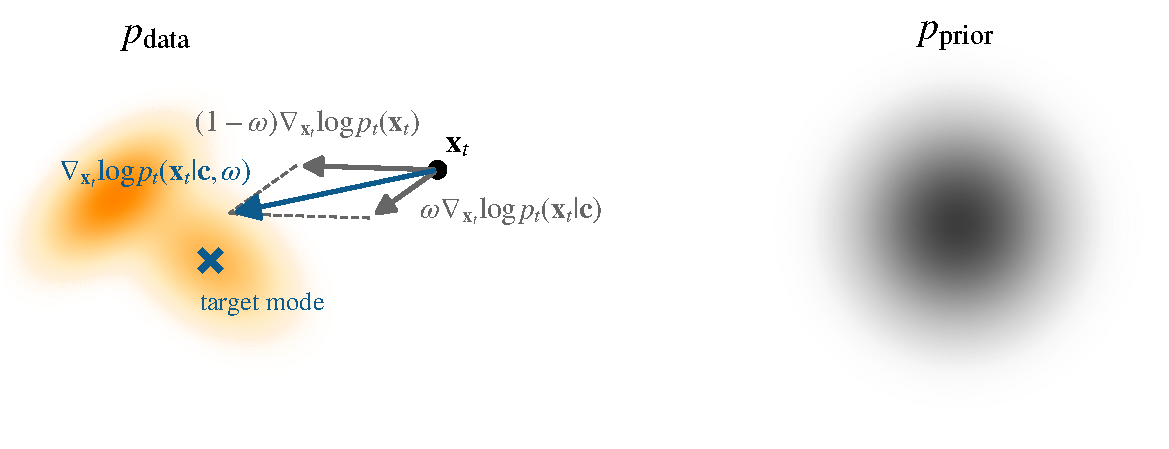
\includegraphics[width=\linewidth]{Images/PartB/classifier_guidance_v2.pdf}
    \caption{\textbfs{Illustration of CFG.} The adjusted score $\nabla_{\rvx_t} \log p_t(\rvx_t| \rvc, \omega)$ is obtained as a linear interpolation between the unconditional score $\nabla_{\rvx_t} \log p_t(\rvx_t)$ and the conditional score $\nabla_{\rvx_t} \log p_t(\rvx_t| \rvc)$, weighted by $\omega$. The resulting direction steers samples from the prior toward modes of the data distribution consistent with the target condition. \figcredit{Created by the authors.}}
    \label{fig:cfg}
\end{figure}

\emph{Classifier-free guidance} (CFG)~\citep{ho2021classifier} is a simplified approach to classifier-based guidance that eliminates the need for a separate classifier. The key idea is to modify the gradient of the score function in a way that allows for effective conditioning without explicit classifiers. Specifically, the gradient of the log-probability of the conditional distribution is adjusted as follows:
\begin{align}
    \nabla_{\rvx_t} \log p_t(\rvc | \rvx_t) = \nabla_{\rvx_t} \log p_t(\rvx_t | \rvc) - \nabla_{\rvx_t} \log p_t(\rvx_t).
\end{align}
Substituting this expression into \Cref{eq:cg_omega} yields the following formulation for the conditioned score:
\begin{align}\label{eq:cfg-model}
\nabla_{\rvx_t} \log p_t(\rvx_t | \rvc, \omega)
&= \nabla_{\rvx_t} \log p_t(\rvx_t) + \omega \left( \nabla_{\rvx_t} \log p_t(\rvx_t | \rvc) - \nabla_{\rvx_t} \log p_t(\rvx_t) \right) \nonumber\\
&= \omega \underbrace{\nabla_{\rvx_t} \log p_t(\rvx_t | \rvc)}_{\text{conditional score}} + (1 - \omega) \underbrace{\nabla_{\rvx_t} \log p_t(\rvx_t)}_{\text{unconditional score}}.
\end{align}

The hyperparameter $\omega$ again plays a critical role in controlling the influence of the conditioning information (we take $\omega \ge 0$):
\begin{itemize}
    \item At $\omega = 0$, the model behaves as an unconditional diffusion model, completely ignoring the conditioning.
    \item At $\omega = 1$, the model uses the conditional score without additional guidance.
    \item For $\omega > 1$, the model places more emphasis on the conditional score and less on the unconditional score, strengthening alignment with $\rvc$ but typically reducing diversity.
\end{itemize}

\subsection{Training and Sampling of CFG}


\paragraph{Joint Training of Unconditional and Conditional Diffusion Models via CFG.} Unlike CG, CFG requires retraining a diffusion model that explicitly accounts for the conditioning variable $\rvc$. Training two separate models for the conditional and unconditional score functions, however, is often computationally prohibitive. To address this, CFG adopts a single model $\mathbf{s}_{\bm{\phi}}(\rvx_t, t; \rvc)$ that learns both score functions within a single model by treating $\rvc$ as an additional input. The training procedure is defined as follows:
\begin{itemize}
    \item For unconditional training, a null token $\emptyset$ is passed in place of the conditioning input, yielding $\rvs_{\bm{\phi}}(\rvx_t, t, \emptyset)$.
    \item For conditional training, the true conditioning variable $\rvc$ is provided as input, resulting in $\rvs_{\bm{\phi}}(\rvx_t, t, \rvc)$.
\end{itemize}
These two training regimes are unified by randomly replacing $\rvc$ with the null input $\emptyset$ with probability $p_\mathrm{uncond}$ (a user-defined hyperparameter typically set to $0.1$). This joint training strategy enables the model to simultaneously learn both conditional and unconditional score functions. The full training algorithm is presented in \Cref{alg:cfg_training}, alongside a comparison to standard unconditional training shown in \Cref{alg:no_cfg_training}. We remark that during training, the CFG weight $\omega$ is not utilized.

\begin{center}
\begin{minipage}[t]{0.48\textwidth}
  \begin{algorithm}[H]
  {\small
    {\small \caption{Uncond. DM \label{alg:no_cfg_training} }}
    \begin{algorithmic}[1]
      \Repeat
        \State $\rvx \sim p_{\text{data}}(\rvx)$
        \State $t \sim \mathcal{U}[0, T]$
        \State $\bm{\epsilon} \sim \mathcal{N}(\mathbf{0}, \mathbf{I})$
        \State $\rvx_t = \alpha_t \rvx + \sigma_t \bm{\epsilon}$
        \State Take gradient step on:
        \Statex \quad $\nabla_{\bm{\phi}} \left\| \rvs_{\bm{\phi}}(\rvx_t, t) - \rvs \right\|^2$
      \Until{converged}
    \end{algorithmic}
    }
  \end{algorithm}
\end{minipage}
\hfill
\begin{minipage}[t]{0.48\textwidth}
  \begin{algorithm}[H]
      {\small
    {\small \caption{CFG for Cond. DM \label{alg:cfg_training}}}
    \begin{algorithmic}[1]
      \Require \textcolor{orange}{$p_\mathrm{uncond}$: prob. of unconditional dropout}
      \Repeat
        \State \textcolor{orange}{$(\rvx, \rvc) \sim p_{\text{data}}(\rvx, \rvc)$}
        \State \textcolor{orange}{$\rvc \gets \emptyset$ with prob. $p_\mathrm{uncond}$}
        \State $t \sim \mathcal{U}[0, T]$
        \State $\bm{\epsilon} \sim \mathcal{N}(\mathbf{0}, \mathbf{I})$
        \State $\rvx_t = \alpha_t \rvx + \sigma_t \bm{\epsilon}$
        \State Take gradient step on:
        \Statex \quad \textcolor{orange}{$\nabla_{\bm{\phi}} \left\| \rvs_{\bm{\phi}}(\rvx_t, t, \rvc) - \rvs \right\|^2$}
      \Until{converged}
    \end{algorithmic}
    }
  \end{algorithm}
\end{minipage}
\end{center}

\paragraph{Conditioned Sampling with CFG.}

Once the model $\rvs_{\bm{\phi}^\times}(\rvx_t, t, \rvc)$ is trained using Algorithm~\ref{alg:cfg_training}, the CFG can be applied during sampling. The gradient of the log-probability is given by:
\begin{align}\label{eq:cfg-model-nn}
\nabla_{\rvx_t} \log p_t(\rvx_t | \rvc, \omega)
&= \omega \nabla_{\rvx_t} \log p_t(\rvx_t | \rvc) + (1 - \omega) \nabla_{\rvx_t} \log p_t(\rvx_t) \nonumber\\
&\approx \omega \underbrace{\rvs_{\bm{\phi}^\times}(\rvx_t, t, \rvc)}_{\text{conditional score}} + (1 - \omega) \underbrace{\rvs_{\bm{\phi}^\times}(\rvx_t, t, \emptyset)}_{\text{unconditional score}}\\
&=: \rvs_{\bm{\phi}^\times}^{\text{CFG}}(\rvx_t ,t, \rvc; \omega). \nonumber
\end{align}

During sampling, a fixed (or optionally time-dependent) classifier-free guidance weight $\omega$ is applied. The unconditional score $\nabla_{\rvx_t} \log p_t(\rvx_t)$ in the reverse-time SDE (\Cref{eq:sde_backward}) or PF-ODE (\Cref{eq:fp_general}) is then replaced by the guided score $\rvs_{\bm{\phi}^\times}^{\mathrm{CFG}}(\rvx_t ,t, \rvc; \omega)$ as in \Cref{eq:condition_prob_ode}, which combines the conditional and unconditional scores in a weighted manner. 

This formulation enables controllable generation by adjusting $\omega$, allowing samples to be guided toward the conditioning signal $\rvc$ while retaining diversity. CFG thus offers an effective and computationally efficient way to achieve precise conditional generation, as it requires training only a single diffusion model.

% \msg{Score Decomposition via Bayes' Rule for Guided Generation}{A key idea behind both CG and CFG is the decomposition of the conditional score into two parts: an unconditional term and a guidance term. This identity follows directly from Bayes' rule (see \Cref{eq:cg_bayes}) and provides a general way to guide diffusion models using auxiliary information. We restate this important formula below, where $\rvy$ denotes the additional information:
% \begin{mdframed}
%     \begin{align}
% \nabla_{\rvx_t} \log p(\rvx_t | \rvy) = \underbrace{\nabla_{\rvx_t} \log p_t(\rvx_t)}_{\text{uncond. direction}} 
% + \underbrace{\nabla_{\rvx_t} \log p_t(\rvy | \rvx_t)}_{\text{guidance direction}}. \label{eq:guidance_bayes}
% \end{align}
% \end{mdframed}

% This decomposition makes it possible to use diffusion models in many ways by approximating the guidance term $\nabla_{\rvx_t} \log p_t(\rvy | \rvx_t)$ based on the application. For example, it enables controllable generation by steering samples toward desired attributes $\rvy$, solves inverse problems at test time using observed measurements, and allows one trained model to handle different tasks by applying suitable guidance signals.


% }

\clearpage
\newpage





\section{Training-Free Guidance}
In this section, we present the high-level philosophy underlying a wide range of training-free guidance methods~\citep{chung2023diffusion,ye2024tfg,he2024manifold,bansal2023universal}. Despite variations in implementation and application, these methods are unified by the central principle expressed in \Cref{eq:guidance_bayes}. We first introduce the high-level approach of training-free guidance in \Cref{subsec:tfg} and then extend this idea to training-free inverse problem solving, with a brief overview provided in \Cref{subsec:inverse-problem}.


\paragraph{Setup and Notations.} Let $\rvc$ denote a conditioning variable. We assume access to a pre-trained diffusion model $\rvs_{\bm{\phi}^\times}(\rvx_t, t)$ expressed in score prediction\footnote{Here, we adopt the score and $\rvx$-prediction parameterization for simplicity of mathematical expression; other parameterizations (e.g., $\beps$-prediction) can be handled analogously.}. In addition, suppose we are given a non-negative function 
\[
\ell(\cdot, \rvc) \colon \mathbb{R}^D \to \mathbb{R}_{\geq 0}
\]
that quantifies how well a sample $\rvx \in \mathbb{R}^D$ aligns with the condition $\rvc$, where smaller values of $\ell(\rvx, \rvc)$ indicate stronger alignment. Concrete examples of such a function include: (i) $\rvc$ is a reference image, and $\ell(\cdot, \rvc)$ is a similarity score measuring perceptual closeness; (ii) $\ell(\cdot, \rvc)$ is a feature-based similarity score computed via a pre-trained model such as CLIP~\citep{radford2021learning}.


Consider the standard linear–Gaussian forward noising kernel 
 $p_{t}(\cdot| \rvx_0):=\mathcal{N}\big(\cdot; \alpha_t\rvx_0, \sigma^2_t\mathbf{I}\big)$.
We recall the DDIM update in \Cref{eq:ddim-update-all} and take it as an example:
\begin{align}\label{eq:ddim-update-clean-noise-score}
\begin{aligned}
    \rvx_{t \rightarrow t-1} =\alpha_{t-1} \underbrace{\hat{\rvx}_0(\rvx_t)}_{\text{in data space}} - \sigma_{t-1} \sigma_t \underbrace{\hat{\rvs}(\rvx_t)}_{\text{in noise space}},
\end{aligned}
\end{align}
where $\hat{\rvx}_0(\rvx_t):=\rvx_{\bm{\phi}^\times}(\rvx_t, t)$ is the (clean) $\rvx$-prediction, and $\hat{\rvs}(\rvx_t):=\rvs_{\bm{\phi}^\times}(\rvx_t, t)$ as the score-prediction from $\rvx_t$ at time level $t$.

\subsection{Conceptual Framework for Training-Free Guidance}\label{subsec:tfg}
Most training-free guidance methods~\citep{ye2024tfg} introduce corrections either in the \emph{data space} or the \emph{noise space} to steer the DDIM update in \Cref{eq:ddim-update-clean-noise-guide} toward satisfying the condition $\rvc$:
\begin{align}\label{eq:ddim-update-clean-noise-guide}
\begin{aligned}
    \rvx_{t \rightarrow t-1} &=\alpha_{t-1} \underbrace{\left(\hat{\rvx}_0(\rvx_t) + {\color{orange}\eta_t^{\text{data}}\mathcal{G}_0} \right)}_{\text{A. data space}} 
    - \sigma_{t-1} \sigma_t \underbrace{\left(\hat{\rvs}(\rvx_t) + {\color{orange}\eta_t^{\text{latent}}\mathcal{G}_t} \right)}_{\text{B. noise space}},
\end{aligned}
\end{align}
where $\eta_t^{\text{data}}, \eta_t^{\text{latent}} \geq 0$ are time-dependent guidance strengths, and $\mathcal{G}_0$, $\mathcal{G}_t$ are correction terms defined below.

\paragraph{A. Guidance in Data Space.}  
By descending along the negative gradient direction 
\[
\mathcal{G}_0 := -\nabla_{\rvx_0} \ell(\rvx_0, \rvc),
\]
the modified clean estimate in data space,
\[
\hat{\rvx}_0(\rvx_t) + {\color{orange}\eta_t^{\text{data}} \mathcal{G}_0},
\]
can be gradually steered toward samples that better satisfy the condition $\rvc$. This gradient-descent scheme can be applied iteratively to progressively improve alignment.

Representative examples include MGPD~\citep{he2023manifold} and UGD~\citep{bansal2023universal}.


% This strategy can also be interpreted as the conditional score decomposition \Cref{eq:guidance_bayes}.

% \begin{align*}
% \nabla_{\rvx_t} \log p_t(\rvx_t|\rvc) 
% &= \underbrace{\nabla_{\rvx_t} \log p_t(\rvx_t)}_{\text{unconditional}} 
% + \underbrace{\nabla_{\rvx_t} \log p(\rvc|\rvx_t)}_{\text{guidance}} 
% \\&\approx \rvs_{\bm{\phi}^\times}(\rvx_t,t) + \eta_t^{\text{latent}} \mathcal{G}_t,
% \end{align*}
% \[
% p(\rvc|\rvx_0) \propto \ell(\rvx_0, \rvc),
% \]
% viewing $\ell_\rvc$ as a surrogate likelihood on the clean signal.

\paragraph{B. Guidance in Noise Space.}  
As discussed in \Cref{sec:prologue-guidance}, the conditional score $\nabla_{\rvx_t} \log p_t(\rvc|\rvx_t)$ is generally intractable. A practical approximation is to introduce a surrogate likelihood $\widetilde p_t(\mathbf{c}|\mathbf{x}_t)$:
\[
\widetilde p_t(\mathbf{c}|\mathbf{x}_t) \propto \exp \big(-\eta\ell \left(\hat{\rvx}_0(\rvx_t), \rvc\right)\big)
\]
with a re-scaling constant $\eta>0$ so that
\[
\nabla_{\rvx_t}\log \widetilde p_t(\mathbf{c}|\mathbf{x}_t) = -\eta\nabla_{\rvx_t}\ell \left(\hat{\rvx}_0(\rvx_t), \rvc\right) =: \mathcal{G}_t,
\]
where $\hat{\rvx}_0(\rvx_t)$ is obtained via the diffusion model's prediction. 
% Then, the guidance direction becomes
% \[
% \nabla_{\rvx_t} \log p_t(\rvc | \rvx_t) 
% \approx \nabla_{\rvx_t} \log \ell_\rvc\left(\hat{\rvx}_0(\rvx_t)\right) 
% =:\mathcal{G}_t.
% \]
Plugging this into the Bayes rule for conditional scores yields the proxy:
\begin{align*}
\nabla_{\rvx_t} \log p_t(\rvx_t|\rvc) 
&\approx \underbrace{\nabla_{\rvx_t} \log p_t(\rvx_t)}_{\text{unconditional}} 
+ \underbrace{\nabla_{\rvx_t} \log \widetilde p_t(\mathbf{c}|\mathbf{x}_t)}_{\text{guidance}} 
\\&\approx \hat{\rvs}(\rvx_t) + \eta_t^{\text{latent}} \mathcal{G}_t,
\end{align*}
which serves as the correction with the guidance in the noise spaces.


However, we note that evaluating $\mathcal{G}_t$ requires backpropagation through the $\rvx$-prediction, i.e.,
\[
\nabla_{\rvx_t} \hat{\rvx}_0(\rvx_t)^\top \cdot 
\left.\nabla_{\rvx_0} \log \ell_{\rvc}(\rvx_0)\right|_{\rvx_0 = \hat{\rvx}_0(\rvx_t)},
\]
which may result in substantial computational cost in practice.

Representative examples include \citep{yu2023freedom, chung2022diffusion, bansal2023universal}.




\subsection{Examples of Training-Free Approaches to Inverse Problems}\label{subsec:inverse-problem}
The principle introduced in \Cref{subsec:tfg} has important applications in inverse problems. We begin with an overview of the background and then provide several concrete examples illustrating how to leverage pre-trained diffusion models for inference-time inverse problem solving.

\paragraph{Background on Inverse Problems.}
Let $\mathcal{A}$ be a corruption operator (which may be linear or nonlinear, known or unknown), such as a blurring kernel or inpainting, and let $\mathbf{y}$ be an observation generated by the following corruption model:
\begin{align}\label{eq:inverse_problem}
    \mathbf{y} = \mathcal{A}(\mathbf{x}_0) + \sigma_{\mathbf{y}} \mathbf{z}, \quad \mathbf{z} \sim \mathcal{N}(\mathbf{0}, \mathbf{I}).
\end{align}
The objective of inverse problems is to sample from the posterior distribution $p_0(\mathbf{x}_0 | \mathbf{y})$, where there may exist infinitely many possible reconstructions $\mathbf{x}_0$ corresponding to the given observation $\mathbf{y}$. The goal is to recover an $\mathbf{x}_0$ that removes the corruptions in $\mathbf{y}$ while preserving its faithful and semantic features.


Traditional approaches to solving inverse problems typically follow a supervised framework, which requires collecting paired data of corrupted and restored samples $(\mathbf{y}, \mathbf{x})$ and relies on optimization methods or supervised training of neural networks. Such approaches can be costly in terms of data preparation and may lack generalization to unseen data.


\paragraph{Pre-Trained Diffusion Models as Inverse Problems Solvers.}
As previously shown, the conditional score can be decomposed via Bayes' rule:
\begin{align}
 \nabla_{\rvx_t} \log p_t(\rvx_t | \rvy) = \underbrace{\nabla_{\rvx_t} \log p_t(\rvx_t)}_{\text{data score}} + \underbrace{\nabla_{\rvx_t}\log p_t(\rvy | \rvx_t)}_{\text{measurement alignment}}.
\label{eq:bayes_rule}
\end{align}

This decomposition separates the data score and a measurement alignment term with $\rvy$ specific to the inverse problem. It enables solving \Cref{eq:inverse_problem} in an unsupervised manner by modeling the clean data distribution $ p_{\text{data}} $ and applying it during inversion. More specifically:
\begin{itemize}
    \item \textbfs{Data score $\nabla_{\rvx_t} \log p_t(\rvx_t)$:} Approximated using a pre-trained diffusion model $\rvs_{\bm{\phi}^\times}(\rvx_t, t)$ trained on clean data.
    \item \textbfs{Measurement alignment $\nabla_{\rvx_t} \log p_t(\rvy | \rvx_t)$:} Intractable in closed form, as it involves marginalizing over latent variables.
\end{itemize}

Consequently, most training-free approaches using pre-trained diffusion models focus on approximating $\nabla_{\rvx_t} \log p_t(\rvy | \rvx_t)$. We adopt a common meta-form summarized in~\citep{daras2024survey}:
\begin{equation*}
    \nabla_{\rvx_t} \log p_t(\rvy | \rvx_t) \approx - \frac{\eqnmarkbox[Plum]{proj}{\mathcal{P}_t}  \, \eqnmarkbox[NavyBlue]{merror}{    \mathcal{M}_t    }}{\eqnmarkbox[OliveGreen]{guidance}{  \gamma_t  }}.
\end{equation*}
Here:
\begin{itemize}
    \item $\mathcal{M}_t$: error vector quantifying the mismatch between the observation $\rvy$ and the estimated signal,
    \item $\mathcal{P}_t$: a mapping that projects $\mathcal{M}_t$ back to the ambient space of $\rvx_t$,
    \item $\gamma_t$: scalar controlling the guidance strength.
\end{itemize}

Representative methods instantiate $\mathcal{M}_t$, $\mathcal{P}_t$, and $\gamma_t$ differently, as highlighted below with color-coded components.

\paragraph{Instantiations of Diffusion-Based Inverse Problem Solvers.}
We present representative methods that leverage a pre-trained diffusion model to provide unsupervised approaches (requiring no paired data) that can be flexibly applied to various inverse problems using the same learned proxy for $ p_{\mathrm{data}} $.


\subparagraph{Score SDE~\citep{song2020score}.} One of the earliest works on diffusion-based inverse problem solvers. It considers a known linear corruption model $\rmA$ and focuses on the noiseless setting with $\sigma_{\rvy} = 0$. Since $\rmA$ is linear, one can form a noise-level–matched observation
\[
\rvy_t := \alpha_t \rvy + \sigma_t \bm{\epsilon},
\]
and use the residual $\rvy_t - \rmA \rvx_t$ (note: $\rvy_t \neq \rmA\rvx_t$ in general) to drive a likelihood-style correction. A common approximation (dropping the multiplicative constant) is
\begin{align*}
    \nabla_{\rvx_t} \log p_t(\rvy|\rvx_t) \approx - \eqnmarkbox[Plum]{proj}{\rmA^\top} (\eqnmarkbox[NavyBlue]{noisymeasurements}{\rvy_t - \rmA \rvx_t}).
\end{align*}

\subparagraph{Iterative Latent Variable Refinement (ILVR)~\citep{choi2021ilvr}.} Using the same setup as ScoreSDE's case, ILVR estimates:
\begin{align*}
    \nabla_{\rvx_t} \log p_t(\rvy| \rvx_t) \approx -\rmA^\dagger(\rvy_t - \rmA\rvx_t) = -\eqnmarkbox[Plum]{moore}{(\rmA^\top \rmA)^{-1} \rmA^\top} (\eqnmarkbox[NavyBlue]{merror}{\rvy_t - \rmA\rvx_t}),
\end{align*}
where $\rmA^\dagger$ is the Moore–Penrose pseudoinverse, and $\rvy_t = \alpha_t\rvy + \sigma_t \bm{\epsilon}_t$.
\subparagraph{Diffusion Posterior Sampling (DPS)~\citep{chung2022diffusion}.} A widely used method for inverse problems with known nonlinear forward operator $\mathcal{A}$ and additive Gaussian noise level $\sigma_{\rvy} \ge 0$ is \emph{Denoising Posterior Score} (DPS), which approximates
\begin{align}\label{eq:dps-score}
  \nabla_{\rvx_t} \log p_t(\rvy|\rvx_t)
   \approx 
  \nabla_{\rvx_t} \log p_t\bigl(\rvy|X_0 = \hat\rvx_0(\rvx_t)\bigr),
\end{align}
where $\hat\rvx_0(\rvx_t) := \E[\rvx_0|\rvx_t]$ denotes the conditional mean of the clean sample given the noisy observation $\rvx_t$ at time $t$, and is typically estimated using Tweedie’s formula (\Cref{eq:tweedie}) from a pre-trained diffusion model. 

This one-point approximation assumes that the conditional distribution $p(\rvx_0|\rvx_t)$ is sharply concentrated, and follows from:
\begin{align*}
  p_t(\rvy|\rvx_t)
  &= \int p_t(\rvy|\rvx_t, \rvx_0)  p(\rvx_0|\rvx_t)  \mathrm{d}\rvx_0 \\
  &= \int p_t(\rvy|\rvx_0)  p(\rvx_0|\rvx_t)  \mathrm{d}\rvx_0 
   \approx  p_t\bigl(\rvy|X_0=\hat\rvx_0(\rvx_t)\bigr),
\end{align*}
where we have used that $\rvy$ depends only on $\rvx_0$ (not on $\rvx_t$) given $\rvx_0$, and the approximation holds under the assumption that the posterior $p(\rvx_0|\rvx_t)$ is tightly peaked around its mean.

Since 
\[
  p_t\bigl(\rvy|X_0 = \hat\rvx_0(\rvx_t)\bigr)
  = \mathcal{N}\bigl(\rvy;  \mathcal{A}(\hat\rvx_0(\rvx_t)),  \sigma_{\rvy}^2 \rmI\bigr),
\]
we compute
\begin{align*}
  \nabla_{\rvx_t} \log p_t(\rvy|\rvx_t)
  &\approx \nabla_{\rvx_t} \log \mathcal{N}\bigl(\rvy;  \mathcal{A}(\hat\rvx_0),  \sigma_{\rvy}^2 \rmI\bigr) \\
  &= -\frac{1}{2\sigma_{\rvy}^2}  \nabla_{\rvx_t} \bigl\| \rvy - \mathcal{A}(\hat\rvx_0) \bigr\|^2 \quad  \\
  &= \frac{1}{\sigma_{\rvy}^2}  \left[ \mathcal{J}_{\mathcal{A}}\big(\hat\rvx_0(\rvx_t)\big) \cdot \nabla_{\rvx_t} \hat\rvx_0(\rvx_t) \right]^\top \bigl( \rvy - \mathcal{A}\big(\hat\rvx_0(\rvx_t)\big) \bigr),
\end{align*}
where $\mathcal{J}_{\mathcal{A}}\big(\hat\rvx_0(\rvx_t)\big) := \nabla_{\rvx_0} \mathcal{A}(\rvx) \big|_{\rvx = \hat\rvx_0(\rvx_t)}$ denotes the Jacobian of the forward operator with respect to its input. This formula propagates the gradient through the score approximation pipeline, reflecting how the measurement likelihood changes with respect to perturbations in the noisy sample $\rvx_t$.

For linear inverse problems, this further simplifies to:
\begin{align*}
    \nabla_{\rvx_t} \log p_t(\rvy | \rvx_t) \approx \eqnmarkbox[OliveGreen]{guidance}{\frac{1}{\sigma_{\rvy}^2}}  \,  \eqnmarkbox[Plum]{proj}{\left[ \rmA \cdot \nabla_{\rvx_t} \hat\rvx_0(\rvx_t) \right]^\top} \left(\eqnmarkbox[NavyBlue]{merror}{\rvy - \rmA(\hat\rvx_0(\rvx_t))}\right).
\end{align*}

A large body of work explores diffusion-based inverse problem solvers by proposing various approximations for $\nabla_{\rvx_t} \log p_t(\rvy | \rvx_t)$.  For a comprehensive overview, we refer readers to the survey by~\citet{daras2024survey}.



\paragraph{A Related Supervised Iterative-Restoration Viewpoint and Its Connection to the PF-ODE.}
The discussion above solves inverse problems by combining a pre-trained diffusion prior with the Bayes-rule decomposition in \Cref{eq:bayes_rule}. More specifically, these methods use the score of the prior distribution together with the measurement model to guide the reconstruction process. At the same time, they also reflect a broader idea: instead of recovering the clean signal in one step, they gradually improve a corrupted input through many small updates. A similar high-level strategy also appears in supervised image restoration, but from a different starting point. Rather than using a pre-trained score model as a prior, these methods learn the refinement procedure directly from paired corrupted and clean examples.

A representative example is InDI~\citep{delbracio2023inversion}. Unlike the Bayes-rule-based approaches above, InDI begins with paired data $(\rvy,\rvx_0)$, where $\rvy$ is a corrupted observation and $\rvx_0$ is the corresponding clean target. Importantly, it does not assume in general that the corruption from $\rvx_0$ to $\rvy$ is known analytically or that it is Gaussian. 

The basic idea is to connect the two endpoints by the interpolation path
\[
\rvx_t=(1-t)\rvx_0+t\rvy,\qquad t\in[0,1].
\]
This path should be understood only as a convenient trajectory from the clean target to the corrupted observation. It is not a Gaussian noising process in general. Along this path, for any $0\le s\le t$, one has the exact relation
\[
\rvx_s=\Bigl(1-\frac{s}{t}\Bigr)\rvx_0+\frac{s}{t}\rvx_t.
\]
Taking conditional expectation given $\rvx_t$ yields
\[
\mathbb E[\rvx_s|\rvx_t]
=
\Bigl(1-\frac{s}{t}\Bigr)\mathbb E[\rvx_0|\rvx_t]
+
\frac{s}{t}\rvx_t.
\]
This shows that, to move from the current state $\rvx_t$ to a slightly less degraded state, it is enough to predict the clean target from $\rvx_t$.

Based on this idea, one trains a time-conditioned predictor $\rmF_{\bphi}(\rvx_t,t)$ from paired examples by minimizing the regression objective
\[
\min_{\bphi}\;
\mathbb E_{(\rvx_0,\rvy)\sim p(\rvx_0,\rvy),\, t\sim p(t)}
\Bigl\|
\rmF_{\bphi}\bigl((1-t)\rvx_0+t\rvy,\,t\bigr)-\rvx_0
\Bigr\|_2^2,
\]
where $p(\rvx_0,\rvy)$ denotes the joint distribution of data pairs consisting of a clean target $\rvx_0$ and its corrupted observation $\rvy$, and $p(t)$ specifies how the interpolation time is sampled during training.
That is, $\rmF_{\bphi}$ is trained to predict the clean target from an intermediate degraded state along the interpolation path. For this squared-error loss, the Bayes-optimal predictor is the conditional expectation
\[
\rmF^*(\rvx_t,t)=\mathbb E[\rvx_0|\rvx_t].
\]
Therefore, if the model class is sufficiently expressive and the optimization is successful, the learned predictor approximates the average clean target associated with the intermediate state $\rvx_t$ at time $t$. In this sense, the training objective is similar in spirit to diffusion-model training: in both cases, one learns a time-conditioned regression from an intermediate corrupted state to a cleaner target. The difference is that diffusion models generate such training pairs synthetically from a prescribed forward corruption process, whereas here the endpoint pairs $(\rvy,\rvx_0)$ come directly from supervised restoration data.

At inference time, one starts from $\hat{\rvx}_1=\rvy$ and repeatedly refines the estimate by
\[
\hat{\rvx}_{t-\Delta t}
=
\frac{\Delta t}{t}\rmF_{\bphi}(\hat{\rvx}_t,t)
+
\Bigl(1-\frac{\Delta t}{t}\Bigr)\hat{\rvx}_t.
\]
Hence, the final reconstruction is produced by gradual refinement rather than by a single direct prediction. In the continuous-time limit, this leads to InDI's residual-flow ODE
\[
\frac{\diff \rvx_t}{\diff t}
=
\frac{\rvx_t-\rmF_{\bphi}(\rvx_t,t)}{t}.
\]

Now suppose we further specialize to the Gaussian denoising setting, where the corruption is assumed to take the known analytic form
\[
\rvy=\rvx_0+\sigma\beps,
\qquad \beps\sim\mathcal N(\bm 0,\rmI),
\]
with known noise level \(\sigma\). Under this specialization, InDI's residual-flow ODE reduces exactly to the probability-flow ODE. Indeed, the interpolation path becomes
\[
\rvx_t=(1-t)\rvx_0+t\rvy
=
\rvx_0+t\sigma\beps,
\]
which is precisely the standard diffusion form
\[
\rvx_t=\alpha_t\rvx_0+\sigma_t\beps,
\qquad\text{with}\qquad
\alpha_t=1,\;\sigma_t=t\sigma.
\]
Therefore, the predictor \(\rmF_{\bphi}(\rvx_t,t)\approx \mathbb E[\rvx_0\mid \rvx_t]\) is now learning to denoise a Gaussian-corrupted intermediate state \(\rvx_t\). In this case, the residual-flow ODE becomes
\[
\frac{\diff \rvx_t}{\diff t}
=
\frac{\rvx_t-\mathbb E[\rvx_0\mid \rvx_t]}{t}
=
-\dot{\sigma}_t\sigma_t\nabla_{\rvx_t}\log p_t(\rvx_t),
\]
where the last equality follows from \(\sigma_t=t\sigma\) together with Tweedie's formula,
\[
\mathbb E[\rvx_0\mid \rvx_t]
=
\rvx_t+\sigma_t^2\nabla_{\rvx_t}\log p_t(\rvx_t).
\]
This is exactly the PF-ODE for this Gaussian denoising path, written in either denoiser form or score form. Thus, under the Gaussian denoising specialization, InDI suggests an alternative interpretation of diffusion modeling: one may view it as supervised denoiser learning on Gaussian-corrupted data, with the PF-ODE arising as the continuous-time limit of gradual refinement.



\newpage
\section{From Reinforcement Learning to Direct Preference Optimization for Model Alignment}\label{sec:rlhf-dpo}

% In the pursuit of aligning generative models with human intent, the prevailing paradigm has been Reinforcement Learning from Human Feedback (RLHF). While effective, RLHF is a complex, multi-stage process prone to instability. This section introduces \emph{Direct Preference Optimization (DPO)}, a more streamlined and stable method that achieves the same objective without the need for explicit reward modeling or reinforcement learning. We then explore its extension to a different generative class with \emph{Diffusion-DPO}.

% \subsection{The Motivation: Circumventing the Pitfalls of RLHF}

% The goal of alignment is to steer a base, pre-trained model (such as a supervised fine-tuned LLM) to produce outputs that humans prefer. The RLHF framework tackles this in three distinct stages. First, supervised fine-tuning (SFT) trains a base model on a dataset of prompt-response pairs. Second, reward modeling (RM) trains a separate model on human preferences consisting of prompts $\mathbf{c}$ and paired responses, one preferred ($\mathbf{x}_w$, ``winner'') and one dispreferred ($\mathbf{x}_l$, ``loser''), with the reward model $r(\mathbf{c},\mathbf{x})$ assigning higher scalar reward to the winner. Finally, RL fine-tuning optimizes the SFT model (now a policy $\pi$) using an RL algorithm such as PPO, maximizing reward-model scores while being regularized by a KL-divergence penalty that keeps $\pi$ close to the reference distribution.

% Despite its impact, this pipeline suffers from drawbacks: the RL stage is unstable and computationally expensive, involving repeated sampling from the policy; it requires training and hosting multiple large models (SFT, reward, and possibly value models); and it optimizes only a proxy for human preferences, meaning flaws in the reward model can be exploited. This motivates a central question: 
% \begin{question}
%     Can we eliminate explicit reward modeling and the unstable RL process, directly optimizing the model on preference data?
% \end{question}
In the pursuit of aligning generative models with human intent, the prevailing paradigm has been Reinforcement Learning from Human Feedback (RLHF). While effective, RLHF is a complex, multi-stage process that can be unstable. This section introduces \emph{Direct Preference Optimization (DPO)}~\citep{rafailov2023direct}, a more streamlined and stable method that reaches the same goal without explicit reward modeling or reinforcement learning. We then outline its extension to diffusion models via \emph{Diffusion-DPO}~\citep{wallace2024diffusion}.

\subsection{The Motivation: Circumventing the Pitfalls of RLHF}

The goal of alignment is to steer a base, pre-trained model (e.g., an SFT model) toward outputs that humans prefer. RLHF proceeds in three stages. First, \emph{supervised fine-tuning (SFT)} trains a base model on prompt–response pairs. Second, \emph{reward modeling (RM)} fits a model on preference data consisting of prompts $\mathbf{c}$ and paired responses (a preferred ``winner'' $\mathbf{x}_w$ and a dispreferred ``loser'' $\mathbf{x}_l$), learning a scalar $r(\mathbf{c},\mathbf{x})$ with $r(\mathbf{c},\mathbf{x}_w)>r(\mathbf{c},\mathbf{x}_l)$. Third, \emph{RL fine-tuning} optimizes the SFT model (policy $\pi$\footnote{A policy maps a prompt/history (state) to a distribution over responses/actions.}) with an algorithm such as PPO~\citep{schulman2017proximal}, maximizing expected reward from $r$ while regularizing by a KL penalty that keeps $\pi$ close to the reference/SFT distribution.

Despite its impact, this pipeline suffers from drawbacks: the RL stage is unstable and computationally expensive because it is on-policy—each update requires freshly generated samples from the current model; it also requires training and hosting multiple large models (SFT, reward, and sometimes a value model); and it optimizes only a proxy for human preferences, so flaws in the reward model can be exploited. This motivates a central question:
\begin{question}
    Can we eliminate explicit reward modeling and the unstable RL step, directly optimizing the model on preference data?
\end{question}

Direct Preference Optimization (DPO) streamlines alignment by replacing the multi-stage RLHF pipeline with a single, supervised-style step. Instead of training a separate reward model and running unstable RL algorithms like PPO, DPO directly fits the policy to preference pairs using a simple logistic loss, while staying close to a fixed reference model. The key insight is that the KL-regularized RLHF objective can be rewritten so that the log-likelihood ratio between the policy and the reference acts as an implicit reward. This preserves the same regularization toward the reference policy but avoids costly rollouts and explicit reward modeling.

In \Cref{subsec:rlhf-bradley-terry}, we briefly review the RLHF pipeline and its reliance on large reward models and RL fine-tuning. In \Cref{subsec:dpo}, we present DPO, originally proposed for language models, which circumvents reward model training and simplifies alignment fine-tuning. Finally, in \Cref{subsec:diffusion-dpo}, we extend this idea to diffusion models, introducing Diffusion-DPO as a practical and stable alignment method in the generative modeling setting.

\subsection{RLHF: Bradley--Terry View}\label{subsec:rlhf-bradley-terry}


\paragraph{Short Introduction to RLHF.}
RLHF begins with a learned judge: a reward model $r_{\bm\psi}$ that assigns a scalar preference score to candidate responses for the same prompt $\mathbf c$. The dataset $\mathcal D$ consists of pairs $(\tilde{\mathbf x},\mathbf x)$ annotated with a label $y$ indicating whether $\tilde{\mathbf x}$ is preferred over $\mathbf x$. The label can be binary $y\in\{0,1\}$ or a soft value $y\in[0,1]$ obtained by aggregating multiple raters. The training objective is a simple logistic loss
\begin{align}\label{eq:rm-emp}
\begin{aligned}
    \mathcal L_{\mathrm{RM}}(\bm\psi)
=
- \mathbb E_{(\mathbf c,\tilde{\mathbf x},\mathbf x,y)\sim\mathcal D}
\Big[
y &\log \sigma \big(r_{\bm\psi}(\mathbf c,\tilde{\mathbf x})-r_{\bm\psi}(\mathbf c,\mathbf x)\big)
\\ &+(1-y)\log \big(1-\sigma \big(r_{\bm\psi}(\mathbf c,\tilde{\mathbf x})-r_{\bm\psi}(\mathbf c,\mathbf x)\big)\big)
\Big],
\end{aligned}
\end{align}
where $\sigma(u)=1/(1+e^{-u})$. In practice, preference pairs in $\mathcal D$ may originate from various sources: curated responses, model snapshots at different checkpoints, or generations from a pre-trained conditional diffusion model.  
A standard convention is to store them in an ordered format $(\text{winner}, \text{loser})$.  
Under this convention we simply set $y=1$, and \Cref{eq:rm-emp} reduces to the special case (with $\tilde\rvx = \rvx^w$ and $\rvx = \rvx^l$):
\begin{equation}\label{eq:rm-bt}
\mathcal L_{\mathrm{RM}}(\bm\psi)
=
- \mathbb E_{(\mathbf c,\mathbf x_w,\mathbf x_l)\sim\mathcal D}
\Big[\log \sigma \big(r_{\bm\psi}(\mathbf c,\mathbf x_w)-r_{\bm\psi}(\mathbf c,\mathbf x_l)\big)\Big].
\end{equation}


\paragraph{Bradley--Terry View and KL Connection.}
It is standard to interpret
\[
p_{r_{\bm\psi}}(\tilde{\mathbf x}\succ \mathbf x|\mathbf c)
:= \sigma \big(r_{\bm\psi}(\mathbf c,\tilde{\mathbf x})-r_{\bm\psi}(\mathbf c,\mathbf x)\big)
\]
through the Bradley--Terry (BT) model~\citep{bradley1952rank}, which converts two scalar scores into a win probability.  
This formulation highlights two key properties: (i) only the \emph{difference} of scores matters (so $r_{\bm\psi}(\mathbf c,\cdot)$ is shift-invariant), and (ii) the loss pushes the predicted winner’s score above the loser’s score. To see (ii) intuitively, consider one pair with label $y\in\{0,1\}$ and define
\[
\Delta r := r_{\bm\psi}(\mathbf c,\tilde{\mathbf x})-r_{\bm\psi}(\mathbf c,\mathbf x),
\quad
p:=\sigma(\Delta r),\quad \sigma(u)=\tfrac{1}{1+e^{-u}}.
\]
The per-example logistic loss is
\[
\ell=-\big[y\log p+(1-y)\log(1-p)\big].
\]
Then
\[
\frac{\partial \ell}{\partial \Delta r}=\sigma(\Delta r)-y.
\]
Under gradient descent with step size $\eta>0$, the score gap updates as
\[
\Delta r \leftarrow \Delta r-\eta\big(\sigma(\Delta r)-y\big).
\]
Hence, if $y=1$ (``$\tilde{\mathbf x}$ wins''), then $\sigma(\Delta r)-1\le 0$, so $\Delta r$ increases (winner up, loser down); if $y=0$, $\Delta r$ decreases.


Each per-example term in \Cref{eq:rm-emp} can be viewed as the cross-entropy between the observed Bernoulli label and the model’s predicted win probability:
\[
-\big[y\log p_{r_{\bm\psi}}+(1-y)\log(1-p_{r_{\bm\psi}})\big]
= \mathcal D_{\mathrm{KL}} \big(\mathrm{Bern}(y) \big\| \mathrm{Bern}(p_{r_{\bm\psi}})\big)
+ \mathcal H \big(\mathrm{Bern}(y)\big),
\]
where $\mathcal H$ is the entropy of the target Bernoulli distribution.
Averaging over the dataset $\mathcal D$ gives
\begin{align}\label{eq:reward_loss}
    \mathcal L_{\mathrm{RM}}(\bm\psi)
= \mathbb E_{\mathcal D} \Big[\mathcal D_{\mathrm{KL}}\left(\mathrm{Bern}(y) \big\| \mathrm{Bern}(p_{r_{\bm\psi}})\right)\Big]
+ \underbrace{\mathbb E_{\mathcal D} \big[\mathcal H(\mathrm{Bern}(y))\big]}_{\text{independent of }\bm\psi}.
\end{align}
Thus, minimizing the logistic loss is equivalent to minimizing the KL divergence between the empirical Bernoulli distribution of human labels and the model’s predicted Bernoulli distribution. In the binary case ($y\in\{0,1\}$), this equivalence is exact; for soft labels ($y\in[0,1]$), the result holds up to an entropy constant offset. Intuitively, the reward model is trained to adjust its win probabilities until they align with the empirical human win rates observed in the dataset.

From this point onward, we adopt the most common convention where $\mathcal D$ stores pairs in an ordered format: $(\rvx^w, \rvx^l, \rvc) \sim \mathcal D$. Under this convention, the label is always $y=1$, and the loss simplifies to the ordered form given in \Cref{eq:rm-bt}, which we will use in the following discussion.

\paragraph{KL Regularized Policy Optimization (with Fixed Reward).}
With the fitted reward $r:=r_{\bm\psi^\times}$ trained via \Cref{eq:rm-bt}, and a conditional pre-trained diffusion model $p_{\bm{\phi}^\times}(\mathbf x|\mathbf c)$, RLHF then adjusts a learnable policy $\pi_{\bm\theta}(\mathbf x|\mathbf c)$, usually fine-tuned on top of $p_{\bm{\phi}^\times}(\mathbf x|\mathbf c)$, toward higher-reward responses.  
At the same time, the policy is regularized to stay close to a reference model, taken as the pre-trained diffusion model $\pi_{\mathrm{ref}}(\mathbf x|\mathbf c):=p_{\bm{\phi}^\times}(\mathbf x|\mathbf c)$, using a $\mathcal{D}_{\mathrm{KL}}$ penalty:
\begin{equation}\label{eq:rlhf-policy-correct}
\max_{\bm\theta} 
\mathbb E_{\mathbf c\sim p(\mathbf c)}
\Big[
\mathbb E_{\mathbf x\sim \pi_{\bm\theta}(\cdot|\mathbf c)}\big[r_{\bm\psi}(\mathbf c,\mathbf x)\big]
-\beta \mathcal{D}_{\mathrm{KL}} \big(\pi_{\bm\theta}(\cdot|\mathbf c) \big\| \pi_{\mathrm{ref}}(\cdot|\mathbf c)\big)
\Big],
\end{equation}
which makes the two forces explicit: seek samples the judge prefers, but stay close to the pre-trained reference.

We remark that the reward objective in \Cref{eq:rm-bt} uses only labeled pairs and does not require that $\mathcal D$ be generated by the reference model (i,e., the pre-trained conditional diffusion model). While not required, collecting pairs from models close to the intended policy can reduce distribution shift and make the learned reward more reliable in the region where it will be used.

In summary, RLHF proceeds in two stages: first fit the reward $r^*$ by minimizing the loss in \Cref{eq:rm-bt} (equivalently, the expected binary $\mathcal{D}_{\mathrm{KL}}$ in \Cref{eq:reward_loss}); then optimize the policy $\pi^*$ by solving \Cref{eq:rlhf-policy-correct}.


\newpage


% \paragraph{Short Introduction to RLHF.}
% RLHF starts with a learned judge: a reward model $r_{\bm\psi}$ that predicts which of two candidates better matches human preferences. For each prompt $\mathbf c$ we observe a pair $(\mathbf x_w,\mathbf x_l)$ where humans prefer the former. The practical training objective on a dataset $\mathcal D$ of labeled pairs is the sample average
% \begin{equation}\label{eq:rm-emp}
% {\mathcal L}_{\mathrm{RM}}(\bm\psi)
% =
% - \mathbb E_{(\mathbf c,\mathbf x_w,\mathbf x_l)\sim\mathcal D}
% \Big[\log \sigma \big(r_{\bm\psi}(\mathbf c,\mathbf x_w)-r_{\bm\psi}(\mathbf c,\mathbf x_l)\big)\Big],
% \end{equation}
% where $\sigma(u)=1/(1+e^{-u})$. It is standard to interpret the score difference through the Bradley--Terry (BT) model, which maps scores to a win probability
% \[
% p_r(\tilde{\mathbf x}\succ \mathbf x|\mathbf c)
% := \sigma \big(r_{\bm\psi}(\mathbf c,\tilde{\mathbf x})-r_{\bm\psi}(\mathbf c,\mathbf x)\big).
% \]
% This view explains shift invariance of $r_{\bm\psi}(\mathbf c,\cdot)$. In practice, pairs in $\mathcal D$ may come from any pool (curated responses, different checkpoints, baselines) and could be mixed; one can imagine a simple special case where they were proposed by a fixed conditional generator (such as a pre-trained fixed conditional diffusion model $p_{\bm{\phi}^\times}(\mathbf x|\mathbf c)$), but this is not necessary. 

% \paragraph{Equivalence to KL minimization.}
% Let $p_{\mathrm{tgt}}(\mathbf c,\mathbf x,\tilde{\mathbf x})$ denote the (oracle or population) distribution that describes how prompts and candidate pairs are drawn, and let
% $p_{\mathrm{gt}}(\tilde{\mathbf x}\succ \mathbf x|\mathbf c)\in[0,1]$ be the (unknown) human win probability for that pair. The corresponding oracle (population) objective integrates over the random human vote:
% \begin{align}\label{eq:rm-pop}
% \begin{aligned}
%     \mathcal L_{\mathrm{RM}}(\bm\psi)
% = - \mathbb E_{(\mathbf c,\mathbf x,\tilde{\mathbf x})\sim p_{\mathrm{tgt}}}
% \Big[
% & p_{\mathrm{gt}}(\tilde{\mathbf x}\succ \mathbf x|\mathbf c) \log p_r(\tilde{\mathbf x}\succ \mathbf x|\mathbf c) \\
% &+ \big(1-p_{\mathrm{gt}}(\tilde{\mathbf x}\succ \mathbf x|\mathbf c)\big) \log \big(1-p_r(\tilde{\mathbf x}\succ \mathbf x|\mathbf c)\big)
% \Big].
% \end{aligned}
% \end{align}
% This is the cross entropy between $p_{\mathrm{gt}}:=p_{\mathrm{gt}}(\tilde{\mathbf x}\succ \mathbf x|\mathbf c)$ and the BT probability 
% $p_r:=p_r(\tilde{\mathbf x}\succ \mathbf x|\mathbf c)$. 

% Since  the cross-entropy of $p_{\mathrm{gt}}$ and $p_r$, $\mathrm{CE}(p_{\mathrm{gt}},p_r)$, is related to their KL divergence denotes via 
% \begin{align*}
%     \mathrm{CE}(p_{\mathrm{gt}},p_r)&=-p_{\mathrm{gt}}\log p_r-(1-p_{\mathrm{gt}})\log(1-p_r)\\   &=\mathcal{D}_{\mathrm{KL}}(\mathrm{Bern}(p_{\mathrm{gt}}) \| \mathrm{Bern}(p_r))+\mathcal{H}(\mathrm{Bern}(p_{\mathrm{gt}})),
% \end{align*}
% with $\mathrm{Bern}(\cdot)$ denotes the Bernoulli distribution (i.e., binary) and $\mathcal{H}(\cdot)$ denotes the entropy, minimizers of $\mathcal L_{\mathrm{RM}}$ are the same as minimizers of the expected Bernoulli KL:
% \begin{equation}\label{eq:reward_loss}
% \min_{\bm\psi} 
% \mathbb E_{(\mathbf c,\mathbf x,\tilde{\mathbf x})\sim p_{\mathrm{tgt}}}
% \big[\mathcal D_{\mathrm{KL}} \big(\mathrm{Bern}(p_{\mathrm{gt}}) \big\| \mathrm{Bern}(p_r)\big)\big].
% \end{equation}
% Connection to the empirical objective: ${\mathcal L}_{\mathrm{RM}}(\bm\psi)$ in \Cref{eq:rm-emp} is a sample approximation to \Cref{eq:rm-pop}. Concretely, replace the expectation over $p_{\mathrm{tgt}}$ by the sample average over $\mathcal D$, and replace the unknown $p_{\mathrm{gt}}$ by the observed label $y$ (or a soft label from multiple raters): for instance each datum is $(\mathbf c,\mathbf x_w,\mathbf x_l)$ with the winner first, the label is implicit ($y=1$). If one adopts a fixed pre-trained model $p_{\bm{\phi}^\times}(\cdot|\rvc)$ to create $p_{\mathrm{tgt}}(\mathbf c,\mathbf x,\tilde{\mathbf x})$, then $p_{\mathrm{tgt}}(\mathbf c,\mathbf x,\tilde{\mathbf x}) = p(\mathbf c) p_{\bm{\phi}^\times}(\mathbf x|\mathbf c) p_{\bm{\phi}^\times}(\tilde{\mathbf x}|\mathbf c)$, but the KL view and the empirical approximation do not rely on this specific choice.

% Therefore minimizing \Cref{eq:rm-pop} is equivalent to minimizing the expected Bernoulli KL, since the entropy term does not depend on $\bm\psi$. In practice we approximate the population objective by the empirical one in \Cref{eq:rm-emp}: replace the population expectation over $p_{\mathrm{tgt}}$ by the sample average over $\mathcal D$, and replace $p_{\mathrm{gt}}$ by the observed label ($y$ or a soft $\hat p$).


% \newpage


% \paragraph{Short Introduction to RLHF.}
% To see where DPO comes from, it helps to view RLHF as beginning with a learned judge: a reward model that scores which of two candidates better matches human preferences. Concretely, for each prompt (context) $\mathbf c$ we observe a pair $(\mathbf x_w,\mathbf x_l)$ where humans prefer the former. Training the judge is just logistic regression on preference pairs:
% \begin{equation}\label{eq:rm-bt}
% \mathcal L_{\mathrm{RM}}(\bm\psi)
% =
% - \mathbb E_{(\mathbf c,\mathbf x_w,\mathbf x_l)\sim\mathcal D}
% \Big[ \log \sigma \big(r_{\bm\psi}(\mathbf c,\mathbf x_w)-r_{\bm\psi}(\mathbf c,\mathbf x_l)\big) \Big],
% \end{equation}
% where $r_{\bm\psi}$ is the reward model and $\sigma(u)=1/(1+e^{-u})$ is the logistic function.
% Equivalently, one can imagine that the dataset $\mathcal D$ arises by first sampling a prompt $\mathbf c\sim p(\mathbf c)$, then drawing two candidates independently from a fixed pre-trained conditional generator $\pi_{\mathrm{ref}}(\cdot|\mathbf c):=p_{\bm{\phi}^\times}(\cdot|\mathbf c)$ (e.g., a pre-trained conditional diffusion model or its SFT fine-tuned version), and finally labeling the pair according to a (possibly stochastic) human preference probability $p_{\mathrm{gt}}(\tilde{\mathbf x}\succ \mathbf x|\mathbf c)\in[0,1]$. The corresponding population loss is the binary cross-entropy
% \begin{align}\label{eq:rm-pop}
% \begin{aligned}
%     \mathcal L_{\mathrm{RM}}(\bm\psi)
% = - \mathbb E_{\substack{\mathbf c\sim p(\mathbf c)\\ \mathbf x,\tilde{\mathbf x}\sim \pi_{\mathrm{ref}}(\cdot|\mathbf c)}}
% \Big[
% & p_{\mathrm{gt}}(\tilde{\mathbf x}\succ \mathbf x|\mathbf c) \log \sigma \big(r_{\bm\psi}(\mathbf c,\tilde{\mathbf x})-r_{\bm\psi}(\mathbf c,\mathbf x)\big) \\
% &+\big(1-p_{\mathrm{gt}}(\tilde{\mathbf x}\succ \mathbf x|\mathbf c)\big) \log \sigma \big(r_{\bm\psi}(\mathbf c,\mathbf x)-r_{\bm\psi}(\mathbf c,\tilde{\mathbf x})\big)
% \Big].
% \end{aligned}
% \end{align}
% This formulation makes the roles explicit: $p(\mathbf c)$ governs prompts, $\pi_{\mathrm{ref}}=p_{\bm{\phi}^\times}$ proposes candidate responses for each prompt, $p_{\mathrm{gt}}$ captures human preference noise, and the reward model $r_{\bm\psi}$ is trained to predict which candidate wins.

% \paragraph{Reward Model Training via Bradley--Terry View.}
% Each comparison yields a binary outcome: “does $\tilde{\mathbf x}$ win over $\mathbf x$ for the same prompt $\mathbf c$?” 
% The Bradley--Terry (BT) model~\citep{bradley1952rank} is the simplest, shift-invariant way to convert scalar preference ratings (logits) into pairwise win probabilities: the probability of preferring $\tilde{\mathbf x}$ depends only on the difference of their preference ratings. If the trainable reward $r_{\bm\psi}(\mathbf c,\cdot)$ assigns higher scores to better candidates, BT posits
% \begin{equation*}
% p_r(\tilde{\mathbf x}\succ \mathbf x |\mathbf c)
% = \sigma \big(r_{\bm\psi}(\mathbf c,\tilde{\mathbf x})-r_{\bm\psi}(\mathbf c,\mathbf x)\big),
% \end{equation*}
% so adding any constant to $r_{\bm\psi}$ leaves preferences unchanged.

% Fitting $r_{\bm\psi}$ with \Cref{eq:rm-bt} is exactly maximum likelihood for the BT model on pairwise data. 
% To see this, rewrite \Cref{eq:rm-pop} as a cross-entropy between the ``human win rate''
% $p_{\mathrm{gt}}:=p_{\mathrm{gt}}(\tilde{\mathbf x}\succ \mathbf x|\mathbf c)$ and the BT probability 
% $p_r:=p_r(\tilde{\mathbf x}\succ \mathbf x|\mathbf c)$:
% \[ 
% \mathcal L_{\mathrm{RM}}(\bm\psi)
% =\mathbb E_{\substack{\mathbf c\sim p(\mathbf c)\\ \mathbf x,\tilde{\mathbf x}\sim \pi_{\mathrm{ref}}(\cdot|\mathbf c)}}
%  \Big[ \underbrace{-p_{\mathrm{gt}}\log p_r-(1-p_{\mathrm{gt}})\log(1-p_r)}_{\mathrm{CE}(p_{\mathrm{gt}},p_r)} \Big].
% \]
% Here, $\mathrm{CE}(p_{\mathrm{gt}},p_r)$ denotes the cross-entropy of $p_{\mathrm{gt}}$ and $p_r$. Since 
% \[
% \mathrm{CE}(p_{\mathrm{gt}},p_r)=\mathcal{D}_{\mathrm{KL}}(\mathrm{Bern}(p_{\mathrm{gt}}) \| \mathrm{Bern}(p_r))+\mathcal{H}(\mathrm{Bern}(p_{\mathrm{gt}})),
% \]
% where $\mathrm{Bern}(\cdot)$ denotes the Bernoulli distribution (i.e., binary) and $\mathcal{H}(\cdot)$ denotes the entropy, minimizers of \Cref{eq:rm-pop} are exactly the minimizers of the expected (Bernoulli) KL:
% \begin{equation}\label{eq:reward_loss}
% \min_{\bm\psi} 
% \mathbb E_{\substack{\mathbf c\sim p(\mathbf c)\\ \mathbf x,\tilde{\mathbf x}\sim \pi_{\mathrm{ref}}(\cdot|\mathbf c)}}
% \Big[\mathcal{D}_{\mathrm{KL}}\big(\mathrm{Bern}(p_{\mathrm{gt}}) \big\| \mathrm{Bern}(p_r)\big)\Big],
% \end{equation}
% because $\mathcal{H} \big(\mathrm{Bern}(p_{\mathrm{gt}})\big)$ does not depend on $\bm\psi$.
% In simple words, training the reward model via \Cref{eq:rm-pop} closes the gap between the judge’s opinion ($p_r$) and the human preference ($p_{\mathrm{gt}}$).

% \paragraph{KL Regularized Policy Optimization (with Fixed Reward).}
% With the fitted reward $r:=r_{\bm\psi^\times}$ in hand trained via \Cref{eq:rm-bt}, RLHF then adjusts a learnable policy $\pi_{\bm\theta}(\mathbf x|\mathbf c)$ toward higher-reward responses while keeping it close to a reference $\pi_{\mathrm{ref}}(\mathbf x|\mathbf c):=p_{\bm{\phi}^\times}(\mathbf x|\mathbf c)$ via a $\mathcal{D}_{\mathrm{KL}}$ regularizer:
% \begin{equation}\label{eq:rlhf-policy-correct}
% \max_{\bm\theta} 
% \mathbb E_{\mathbf c\sim p(\mathbf c)}
% \Big[
% \mathbb E_{\mathbf x\sim \pi_{\bm\theta}(\cdot|\mathbf c)}\big[r_{\bm\psi}(\mathbf c,\mathbf x)\big]
% -\beta \mathcal{D}_{\mathrm{KL}} \big(\pi_{\bm\theta}(\cdot|\mathbf c) \big\| \pi_{\mathrm{ref}}(\cdot|\mathbf c)\big)
% \Big],
% \end{equation}
% which makes the two forces explicit: seek samples the judge prefers, but stay close to the pre-trained reference.

% \textit{Clarification.} The reward objective in \Cref{eq:rm-emp} uses only labeled pairs and does not require that $\mathcal D$ be generated by the reference model. By contrast, the policy objective \Cref{eq:rlhf-policy-correct} does require a fixed reference $\pi_{\mathrm{ref}}$ (commonly the pre-trained conditional diffusion model), which defines the KL term and usually initializes $\pi_{\bm\theta}$. While not required, collecting pairs from models close to the intended policy can reduce distribution shift and make the learned reward more reliable in the region where it will be used.




% In summary, RLHF proceeds in two stages: first fit the reward $r^*$ by minimizing the population loss in \Cref{eq:rm-pop} (equivalently, the expected binary $\mathcal{D}_{\mathrm{KL}}$ in \Cref{eq:reward_loss}); then optimize the policy $\pi^*$ by solving \Cref{eq:rlhf-policy-correct}.


\subsection{DPO Framework}\label{subsec:dpo}
\paragraph{The Bridge from RLHF.}
The KL-regularized policy objective in \Cref{eq:rlhf-policy-correct} has a simple closed-form solution for each prompt $\mathbf c$, given the fitted reward $r := r_{\bm\psi^\times}$, expressed in the following energy-based form~\citep{peters2010relative}:
\begin{equation}\label{eq:rlhf-closed-form}
\pi^*(\mathbf x|\mathbf c)
=
\frac{1}{Z(\mathbf c)} \pi_{\mathrm{ref}}(\mathbf x|\mathbf c)\exp(r(\mathbf c,\mathbf x)/\beta),
\end{equation}
where $\pi_{\mathrm{ref}}(\mathbf x|\mathbf c):=p_{\bm{\phi}^\times}(\mathbf x|\mathbf c)$,  and $Z(\mathbf c)$ is the partition function ensuring $\int \pi^*(\mathbf x|\mathbf c) \diff \mathbf x=1$.

For smaller $\beta$, $\exp(r/\beta)$ becomes sharper, so $\pi^*$ concentrates on high reward regions: reward dominates, the policy moves farther from $\pi_{\mathrm{ref}}$, diversity decreases, and training may become unstable or prone to reward hacking. For larger $\beta$, $\exp(r/\beta)$ flattens, keeping $\pi^*$ closer to $\pi_{\mathrm{ref}}$: the KL term dominates, updates are conservative, diversity follows the reference, but reward gains are limited.

Since our aim is to fine-tune the policy directly (without training a separate reward model), \Cref{eq:rlhf-closed-form} lets us \emph{define} an \textit{implicit reward} from any policy. We introduce below:
\paragraph{Defining an Implicit Reward Motivated by Inverting \Cref{eq:rlhf-closed-form}.}
\Cref{eq:rlhf-closed-form} suggests an immediate inversion: for any policy $\pi$ (with support contained in $\pi_{\mathrm{ref}}$), define
\begin{equation}\label{eq:implicit-reward}
r_{\pi}(\mathbf c,\mathbf x)
 = 
\beta \log\frac{\pi(\mathbf x|\mathbf c)}{\pi_{\mathrm{ref}}(\mathbf x|\mathbf c)}
 + \beta \log Z(\mathbf c).
\end{equation}
Then \Cref{eq:rlhf-closed-form} holds with $\pi$ in place of $\pi^*$, i.e., $\pi$ would be the optimizer of \Cref{eq:rlhf-policy-correct} for the reward function $r_{\pi}$.
In this sense, $r_{\pi}$ is an \emph{implicit (policy-induced) reward}: it is identified up to the prompt-dependent constant $\beta\log Z(\mathbf c)$, which vanishes in any pairwise comparison such as in the BT model:
\[
r_{\pi}(\mathbf c,\mathbf x_w)-r_{\pi}(\mathbf c,\mathbf x_l)
=
\beta\Big(
\log\frac{\pi(\mathbf x_w|\mathbf c)}{\pi_{\mathrm{ref}}(\mathbf x_w|\mathbf c)}
-
\log\frac{\pi(\mathbf x_l|\mathbf c)}{\pi_{\mathrm{ref}}(\mathbf x_l|\mathbf c)}
\Big).
\]
This cancellation is exactly what makes the constant irrelevant for preference learning and leads directly to the DPO loss on log-probability differences.

\paragraph{DPO's Training Loss.}
Plug the implicit reward \Cref{eq:implicit-reward} into the BT model of \Cref{eq:rm-bt} for a labeled pair $(\mathbf x_w,\mathbf x_l)$ under the same prompt $\mathbf c$. 
The constants $\log Z(\mathbf c)$ cancel between winner and loser, yielding a single logistic-loss objective on log-probability differences:
\begin{align*}
\mathcal L_{\mathrm{DPO}}(\bm\theta;\pi_{\mathrm{ref}})
&=
-\mathbb E_{(\mathbf c,\mathbf x_w,\mathbf x_l)\sim\mathcal D} \left[
\log \sigma \Big(
\beta\big(
\log\frac{\pi_{\bm\theta}(\mathbf x_w|\mathbf c)}{\pi_{\mathrm{ref}}(\mathbf x_w|\mathbf c)}
-
\log\frac{\pi_{\bm\theta}(\mathbf x_l|\mathbf c)}{\pi_{\mathrm{ref}}(\mathbf x_l|\mathbf c)}
\big)
\Big)
\right].
\end{align*}
In words: DPO pushes up the (temperature-scaled) advantage of the winner over the loser, measured as the difference of log-likelihood improvements over the reference:
\[
-\log \sigma \left(
  \beta 
  \bigl[
    \text{log-ratio difference of }
    \tfrac{\pi_{\bm\theta}}{\pi_{\mathrm{ref}}}
    \text{ at } \mathbf x_w \text{ vs.\ } \mathbf x_l
  \bigr]
\right).
\]
This achieves the goal of RLHF in a single, stable classification-style
fine-tuning stage, without training an explicit reward model.


\subsection{Diffusion-DPO}\label{subsec:diffusion-dpo}
\paragraph{Why Naive DPO Fails for Diffusion Models?}
Evaluating the sample likelihood $\pi_\btheta(\mathbf x|\mathbf c)$ in diffusion models requires the instantaneous change-of-variables formula (divergence of the drift) of ODE solving (see \Cref{eq:score-sde-likelihood})\footnote{In discrete-time diffusion models (e.g., DDPM), evaluating $\pi_{\bm\theta}(\mathbf x_0| \mathbf c)$ requires marginalizing over the latent reverse trajectory $\mathbf x_{1:T}$.
}, which is computationally intensive. Moreover, differentiating through the entire sampling trajectory can suffer from vanishing or exploding gradients. To avoid these issues, Diffusion-DPO works at the \emph{path} level. We take the discrete-time diffusion model (e.g., DDPM) as an illustrative example; the continuous-time diffusion model is analogous.

\paragraph{Defining Pathwise Implicit Rewards.}
Let a trajectory be $\mathbf x_{0:T}:=(\mathbf x_T,\ldots,\mathbf x_0)$ under the reverse-time Markov chain with conditionals $\pi(\mathbf x_{t-1}|\mathbf x_t,\mathbf c)$. Here, $\mathbf x_T$ denotes a sample from the prior (highest noise), and $\mathbf x_0$ is the clean output in data space. Since generation in diffusion models proceeds along a full denoising path, it is natural to extend preferences from final outputs to the entire trajectory. We therefore assign each trajectory a reward $R(\mathbf c,\mathbf x_{0:T})$, which reduces to an endpoint reward if it depends only on $\mathbf x_0$, but can also capture cumulative effects along the path. 

We replace the sample-level KL in \Cref{eq:rlhf-policy-correct} by a pathwise KL as:
\[
\max_{\btheta}\mathbb E_{\mathbf c\sim p(\mathbf c)}
\Big[
\underbrace{\mathbb E_{\mathbf x_{0:T}\sim \pi_{\btheta}(\cdot|\mathbf c)}[R(\mathbf c,\mathbf x_{0:T})]}_{\text{reward over paths}}
-\beta \mathcal D_{\mathrm{KL}} \big(\pi_{\btheta}(\cdot|\mathbf c) \big\| \pi_{\mathrm{ref}}(\cdot|\mathbf c)\big)
\Big],
\]
where $\pi_{\btheta}(\cdot|\mathbf c)$ and $\pi_{\mathrm{ref}}(\cdot|\mathbf c)$ are the \emph{path} distributions. It aims to maximize the reward for reverse process $\pi_{\btheta}(\cdot|\mathbf c)$, while matching the distribution of
the original reference reverse process $\pi_{\mathrm{ref}}(\cdot|\mathbf c)$.

For each prompt $\mathbf c$, the optimizer has the simple energy-based form
\begin{equation}\label{eq:path-closed-form}
\pi^*(\mathbf x_{0:T}|\mathbf c)
=\frac{1}{Z(\mathbf c)} \pi_{\mathrm{ref}}(\mathbf x_{0:T}|\mathbf c) 
\exp \big(R(\mathbf c,\mathbf x_{0:T})/\beta\big),
\end{equation}
with $Z(\mathbf c)$ a normalizer. Inverting \Cref{eq:path-closed-form} motivates the definition of an \emph{implicit path reward} for any policy $\pi$:
\[
R_{\pi}(\mathbf c,\mathbf x_{0:T})
:=\beta\log\frac{\pi(\mathbf x_{0:T}|\mathbf c)}{\pi_{\mathrm{ref}}(\mathbf x_{0:T}|\mathbf c)}+\beta\log Z(\mathbf c),
\]
whose constant $\beta\log Z(\mathbf c)$ is irrelevant for pairwise comparisons.

\paragraph{From Pathwise Implicit Rewards to DPO.}
Apply the Bradley--Terry model to \emph{paths} for a labeled pair $(\mathbf x^w_0,\mathbf x^l_0)$ under the same prompt $\mathbf c$, and use the standard logistic log-loss:
\begin{align}\label{eq:diffusion-dpo}
\begin{aligned}
\mathcal L_{\mathrm{Diff\text{-}DPO}}(\bm\theta;\pi_{\mathrm{ref}})
&:=
- \mathbb E_{(\mathbf c,\mathbf x_0^w,\mathbf x_0^l)\sim\mathcal D}
 \left[\log \sigma \big(\Delta R(\mathbf c;\bm\theta)\big)\right], \quad \text{where}\\
\Delta R(\mathbf c;\bm\theta)
&:=
\underbrace{\mathbb E_{\mathbf x_{1:T}^w\sim \pi_{\bm\theta}(\cdot | \mathbf x_0^w,\mathbf c)}
 \Big[R_{\pi_{\bm\theta}} \big(\mathbf c,(\mathbf x_0^w,\mathbf x_{1:T}^w)\big)\Big]}_{\text{winner path expectation}}
\\ &\quad\quad\quad-
\underbrace{\mathbb E_{\mathbf x_{1:T}^l\sim \pi_{\bm\theta}(\cdot | \mathbf x_0^l,\mathbf c)}
 \Big[R_{\pi_{\bm\theta}} \big(\mathbf c,(\mathbf x_0^l,\mathbf x_{1:T}^l)\big)\Big]}_{\text{loser path expectation}}. 
\end{aligned}
\end{align}
Here, the expectation $\mathbb E_{\mathbf x_{1:T}\sim\pi_{\bm\theta}(\cdot|\mathbf x_0,\mathbf c)}[\cdot]$ means:
given a fixed endpoint $\mathbf x_0$ (e.g., the winner $\mathbf x_0^w$) from the dataset, we take an
expectation over latent denoising trajectories $\mathbf x_{1:T}$ under the model-induced conditional path
distribution (the posterior over reverse-time trajectories) that, with kernels
$\pi_{\bm\theta}(\mathbf x_{t-1}|\mathbf x_t,\mathbf c)$, could produce $\mathbf x_0$.
Since these intermediate states are unobserved, we average the path reward over all such trajectories.


However, \Cref{eq:diffusion-dpo} is impractical for three practical reasons:
\begin{enumerate}[leftmargin=*]
\item \textbfs{Endpoint Conditioning Induces an Intractable Path Posterior.}
The term $\mathbb E_{\pi_{\bm\theta}(\mathbf x_{1:T}|\mathbf x_0,\mathbf c)}[\cdot]$ averages over reverse paths constrained to hit $\mathbf x_0$, whereas the sampler runs $\mathbf x_T \to \cdots \to \mathbf x_0$ without this constraint. Conditioning on the endpoint creates a diffusion-bridge posterior with generally no closed form and costly sampling.

\item \textbfs{Nested, $\bm\theta$-Coupled Expectations.}
The loss $-\log\sigma(\Delta R(\mathbf c;\bm\theta))$ with
\[
\Delta R=\mathbb E_{\text{paths}|\mathbf x_0^w,\mathbf c}[R_{\pi_{\bm\theta}}]
-\mathbb E_{\text{paths}|\mathbf x_0^l,\mathbf c}[R_{\pi_{\bm\theta}}]
\]
has both the path joint distribution and the integrand $R_{\pi_{\bm\theta}}$ depending on $\bm\theta$. Thus $\nabla_{\bm\theta}$ must differentiate through the sampling distribution, leading to REINFORCE/pathwise couplings and high-variance gradients.

\item \textbfs{Long Chains, Large Sums, and Expensive Backpropagation.}
In $R_{\pi_{\bm\theta}}(\mathbf c,\mathbf x_{0:T})$, computing
\[
\beta \left[\log \pi_{\bm\theta}(\mathbf x_{0:T}|\mathbf c)
-\log \pi_{\mathrm{ref}}(\mathbf x_{0:T}|\mathbf c)\right]
\]
requires $\mathcal O(T)$ per-step log-densities with $T \sim 10^2$–$10^3$, for both policy $\pi_{\bm\theta}$ and reference $\pi_{\mathrm{ref}}$, and for both winner/loser paths. Backpropagating through these stochastic chains (or bridge samplers) is memory and compute heavy and can be unstable; repeating this over many samples per pair and across all triplets pushes training beyond practical budgets.
\end{enumerate}

\paragraph{Toward a Tractable Surrogate for \Cref{eq:diffusion-dpo}.}
To make this computable, we apply a key mathematical insight. By leveraging properties of diffusion models and applying Jensen's inequality, we can optimize a tractable upper bound on this loss. This transforms the problem from evaluating an entire path's likelihood to evaluating an expectation over the individual, single-step transitions within the path:

Because $-\log\sigma(\cdot)$ is convex, Jensen’s inequality yields an upper bound by moving the inner expectations outside the nonlinear function:
\begin{align*}
&\mathcal L_{\mathrm{Diff\text{-}DPO}}(\bm\theta;\pi_{\mathrm{ref}})
\\ \le  &
-\mathbb E_{(\mathbf c,\mathbf x_0^w,\mathbf x_0^l)\sim\mathcal D}
  \mathbb E_{\substack{\mathbf x^w_{1:T}\sim \pi_{\bm\theta}(\cdot | \mathbf x_0^w,\mathbf c)\\[1pt]
                       \mathbf x^l_{1:T}\sim \pi_{\bm\theta}(\cdot | \mathbf x_0^l,\mathbf c)}}
\left[
\log \sigma \Big(
R_{\pi_{\bm\theta}}(\mathbf c,\mathbf x^w_{0:T})
-
R_{\pi_{\bm\theta}}(\mathbf c,\mathbf x^l_{0:T})
\Big)
\right].
\end{align*}
Using the implicit-reward identity $R_{\pi_{\bm\theta}}=\beta\log\frac{\pi_{\bm\theta}}{\pi_{\mathrm{ref}}}+\beta\log Z(\mathbf c)$ and cancellation of the constant between winner and loser, the bound becomes
\begin{align}\label{eq:dpo-path-bound}
\mathcal L_{\mathrm{Diff\text{-}DPO}}(\bm\theta;\pi_{\mathrm{ref}})
& \le
-\mathbb E
\left[
\log \sigma \Big(
\beta\big(
\log\frac{\pi_{\bm\theta}(\mathbf x^w_{0:T}| \mathbf c)}{\pi_{\mathrm{ref}}(\mathbf x^w_{0:T}| \mathbf c)}
-
\log\frac{\pi_{\bm\theta}(\mathbf x^l_{0:T}| \mathbf c)}{\pi_{\mathrm{ref}}(\mathbf x^l_{0:T}| \mathbf c)}
\big)
\Big)
\right].
\end{align}

\subparagraph{A Tractable Surrogate (Stepwise Form).} We now exploit the Markov property of the reverse process to decompose the upper bound of $\mathcal L_{\mathrm{Diff\text{-}DPO}}$. This allows us to express the path-level preference as a sum of per-step contributions, converting the intractable pathwise loss into a tractable single-step estimator. The resulting form yields a DPO-style log-sigmoid loss whose inner margin reduces to a DSM-style MSE difference. Concretely, for the reverse chain,
\begin{align*}
    \pi_{\bm\theta}(\mathbf x_{0:T}| \mathbf c)
&=\pi_{\bm\theta}(\mathbf x_T| \mathbf c) \prod_{t=1}^{T}
\pi_{\bm\theta}(\mathbf x_{t-1}| \mathbf x_t,\mathbf c),
\\
\pi_{\mathrm{ref}}(\mathbf x_{0:T}| \mathbf c)
&=\pi_{\mathrm{ref}}(\mathbf x_T| \mathbf c) \prod_{t=1}^{T}
\pi_{\mathrm{ref}}(\mathbf x_{t-1}| \mathbf x_t,\mathbf c).
\end{align*}
Hence
\[
\frac{\pi_{\bm\theta}(\mathbf x_{0:T}| \mathbf c)}{\pi_{\mathrm{ref}}(\mathbf x_{0:T}| \mathbf c)}
=
\frac{\pi_{\bm\theta}(\mathbf x_T| \mathbf c)}{\pi_{\mathrm{ref}}(\mathbf x_T| \mathbf c)}
\prod_{t=1}^{T}
\frac{\pi_{\bm\theta}(\mathbf x_{t-1}| \mathbf x_t,\mathbf c)}
     {\pi_{\mathrm{ref}}(\mathbf x_{t-1}| \mathbf x_t,\mathbf c)}.
\]
If the prior at time $T$ is the same for both models,
$\pi_{\bm\theta}(\mathbf x_T| \mathbf c)=\pi_{\mathrm{ref}}(\mathbf x_T| \mathbf c)$,
then the first factor equals $1$, and taking logs yields
\[
\log\frac{\pi_{\bm\theta}(\mathbf x_{0:T}| \mathbf c)}{\pi_{\mathrm{ref}}(\mathbf x_{0:T}| \mathbf c)}
=\sum_{t=1}^{T}
\log\frac{\pi_{\bm\theta}(\mathbf x_{t-1}| \mathbf x_t,\mathbf c)}
         {\pi_{\mathrm{ref}}(\mathbf x_{t-1}| \mathbf x_t,\mathbf c)}.
\]
It follows that the bound in \Cref{eq:dpo-path-bound} can be written as
\[
\mathcal L_{\mathrm{Diff\text{-}DPO}}(\bm\theta;\pi_{\mathrm{ref}})
  \le  - \E \left[\log\sigma \Big(\beta \sum_{t=1}^T \Delta_t\Big)\right],
\]
where each per-step contribution is
\[
\Delta_t
= \log\frac{\pi_{\bm\theta}(\mathbf x^w_{t-1}|\mathbf x^w_t,\mathbf c)}
               {\pi_{\mathrm{ref}}(\mathbf x^w_{t-1}|\mathbf x^w_t,\mathbf c)}
- \log\frac{\pi_{\bm\theta}(\mathbf x^l_{t-1}|\mathbf x^l_t,\mathbf c)}
               {\pi_{\mathrm{ref}}(\mathbf x^l_{t-1}|\mathbf x^l_t,\mathbf c)}.
\]

To obtain a tractable estimator, we apply a single step Jensen upper bound: sample
$t\sim\mathcal U\{1,\dots,T\}$ (one timestep per training pair) and rescale by $T$. This yields
\[
-\log\sigma \Big(\beta \sum_{t=1}^T \Delta_t\Big)
 \le  \E_{t} \left[-\log\sigma \big(\beta T \Delta_t\big)\right].
\]

Thus the final objective is an expected per-step surrogate,
\[
\mathcal L_{\mathrm{Diff\text{-}DPO}}(\bm\theta;\pi_{\mathrm{ref}})
 \le   
- \E_{\substack{(\mathbf c,\mathbf x_0^w,\mathbf x_0^l)\sim\mathcal D \\[2pt] t\sim \mathcal U\{1,\dots,T\}}}
\left[\log\sigma \big(\beta T  \Delta_t\big)\right],
\]
which reduces the original pathwise loss to a tractable single step upper-bound estimator.

Following the original Diffusion-DPO derivation, we further replace the intractable reverse-process sampling with the forward noising process $q(\mathbf x_t|\mathbf x_0)$. For Gaussian reverse conditionals used in diffusion models (take $\boldsymbol\epsilon$-prediction as an example),
\[
\log\frac{\pi_{\bm\theta}(\mathbf x_{t-1}| \mathbf x_t,\mathbf c)}{\pi_{\mathrm{ref}}(\mathbf x_{t-1}| \mathbf x_t,\mathbf c)}
= \text{Constant}
-\lambda_t \Big(\underbrace{\big\|\hat{\boldsymbol\epsilon}_{\bm\theta}(\mathbf x_t,t,\mathbf c)-\boldsymbol\epsilon\big\|^2}_{\mathrm{policy}}
-\underbrace{\big\|\hat{\boldsymbol\epsilon}_{\mathrm{ref}}(\mathbf x_t,t,\mathbf c)-\boldsymbol\epsilon\big\|^2}_{\mathrm{reference}}\Big),
\]
where $\lambda_t>0$ absorbs noise schedule factors. Thus each per-time contribution is proportional to an MSE difference (policy vs.\ reference) at slice $t$.

For notation simplicity, define for any noised sample $(\mathbf x_t,\boldsymbol\epsilon)$:
\[
\Delta\mathrm{MSE}(\mathbf x_t;\boldsymbol\epsilon)
:= \big\|\hat{\boldsymbol\epsilon}_{\bm\theta}(\mathbf x_t,t,\mathbf c)-\boldsymbol\epsilon\big\|^2
 - \big\|\hat{\boldsymbol\epsilon}_{\mathrm{ref}}(\mathbf x_t,t,\mathbf c)-\boldsymbol\epsilon\big\|^2.
\]

This motivates the following practical single-step Diffusion-DPO surrogate for $\mathcal L_{\mathrm{Diff\text{-}DPO}}(\bm\theta;\pi_{\mathrm{ref}})$:
\begin{mdframed}
\begin{align*}
    &\tilde{\mathcal L}_{\mathrm{Diff\text{-}DPO}}(\bm\theta;\pi_{\mathrm{ref}})
    :=
    \\&-\mathbb E_{\substack{(\mathbf c,\mathbf x_0^w,\mathbf x_0^l)\sim\mathcal D\\
    t\sim\mathcal U\{1,\dots,T\}, \boldsymbol\epsilon^w,\boldsymbol\epsilon^l\sim\mathcal N(\mathbf 0,\mathbf I)}}
    \Big[
    \log\sigma\!\Big(
    w(t)\big(\Delta\mathrm{MSE}(\mathbf x_t^l;\boldsymbol\epsilon^l)-\Delta\mathrm{MSE}(\mathbf x_t^w;\boldsymbol\epsilon^w)\big)
    \Big)
    \Big],
\end{align*}
\end{mdframed}
where $\mathbf x_t^w=\alpha_t \mathbf x_0^w+\sigma_t \boldsymbol\epsilon^w$ and $\mathbf x_t^l=\alpha_t \mathbf x_0^l+\sigma_t \boldsymbol\epsilon^l$, with $\boldsymbol\epsilon^w,\boldsymbol\epsilon^l\sim\mathcal N(\mathbf 0,\mathbf I)$, and $w(t)>0$ absorbs the positive scaling and time weighting factors (e.g., $w(t)\propto \beta T \lambda_t$). In practice, one may also use shared noise $\boldsymbol\epsilon^w=\boldsymbol\epsilon^l$
as a variance-reduction variant; this does not change the overall DPO-style form
of the objective, but slightly alters the stochastic estimator.

Intuitively, minimizing $\tilde{\mathcal L}_{\mathrm{Diff\text{-}DPO}}$ increases the reference-normalized winner-over-loser margin. Equivalently, it encourages the model to reduce denoising error on the winner more than on the loser, measured relative to the frozen reference model. The reference model does not contribute a direct gradient term, but it remains inside the margin within the $\log\sigma(\cdot)$ nonlinearity, so it still shapes the DPO-style per-example weighting.


\newpage
\section{Closing Remarks}\label{sec:ch8_cr}

This chapter has shifted our focus from foundational principles to the practical challenge of controllable generation. We established a unified framework for guidance based on the Bayesian decomposition of the conditional score, which elegantly separates the generative process into an unconditional direction and a steering term.

We saw this principle manifest in several powerful techniques. We covered methods that require dedicated training, such as Classifier Guidance (CG), which uses an external classifier, and the more efficient Classifier-Free Guidance (CFG), which learns conditional and unconditional scores within a single model. We also explored flexible training-free guidance methods, which can steer a pre-trained model at inference time by defining a surrogate likelihood from an arbitrary loss function, enabling applications from artistic control to solving inverse problems without any retraining.

Beyond simple conditioning, we delved into the nuanced task of aligning model outputs with human preferences. After reviewing the standard but complex RLHF pipeline, we introduced Direct Preference Optimization (DPO) and its novel adaptation, Diffusion-DPO, as a more direct and stable alternative. This approach elegantly bypasses the need for an explicit reward model and reinforcement learning by deriving a loss directly from preference data.


Through these techniques, we have assembled a powerful toolkit for steering the generative process. However, a major practical hurdle remains untouched: the significant computational cost and latency of the iterative sampling process itself. Having addressed what to generate, we now turn to the equally important question of how fast we can generate it. The next chapter will tackle this challenge directly:
\begin{enumerate}
    \item We will leverage the insight that sampling is equivalent to solving an ODE to explore sophisticated numerical solvers designed to drastically reduce the number of required steps.
    \item We will investigate a sequence of influential methods, including DDIM, DEIS, and the DPM-Solver family, which have made diffusion models far more practical by accelerating sampling speed by orders of magnitude.
\end{enumerate}

